\documentclass[preprint,12pt,authoryear]{elsarticle}

\usepackage{amsmath,amssymb,amsthm}
\usepackage{booktabs,array}
\usepackage{graphicx}
\usepackage{url}
\usepackage{enumitem}
\usepackage{microtype}
\usepackage{placeins}
\usepackage[labelfont=bf]{caption}
\usepackage{subcaption}
\usepackage{xr-hyper}
\usepackage[colorlinks=true,linkcolor=blue,citecolor=blue,urlcolor=blue]{hyperref}

\journal{Epidemics}

\newtheorem{proposition}{Proposition}
\newtheorem{corollary}{Corollary}
\newtheorem{remark}{Remark}
\newtheorem{definition}{Definition}

\newcommand{\E}{\mathbb{E}}
\newcommand{\Var}{\mathrm{Var}}
\newcommand{\NB}{\mathrm{NB}}
\newcommand{\Bin}{\mathrm{Bin}}
\newcommand{\CV}{\mathrm{CV}}
\newcommand{\Rbar}{\bar{R}}
\newcommand{\mx}{m_\times}

\externaldocument{build/supplement}

\begin{document}

\begin{frontmatter}

\title{Limits to improving reproduction number estimates by increasing case counts: Environmental variability, reporting heterogeneity, and surveillance design}

\author{Chi Wang}
\affiliation{organization={School of Safety Science and Engineering, Xi'an University of Science and Technology},
            city={Xi'an},
            postcode={710054},
            country={China}}

\begin{abstract}
Estimation errors in the reproduction number are frequently attributed to sample size. Here we show that the return on increasing case counts depends fundamentally on the inferential target, distinguishing the conditional instantaneous reproduction number $R_t$ from the cross-period mean $\bar{R}$. Under negative-binomial transmission and binomial reporting, the estimation error of $R_t$ decays as $1/m$ with expected reporting scale $m$, attaining the Cram\'er--Rao bound. For single-period estimators of $\bar{R}$ that are conditionally unbiased for $R_t$, however, the estimation error retains an irreducible variance floor $v_R$ arising from environmental stochasticity, with reporting heterogeneity introducing an additional component $v_H$ into our estimator's variance when reporting probabilities fluctuate across periods. This irreducibility is specific to expanding single-period case volume and does not preclude variance reduction through accumulating independent observation periods. We derive the variance balance scale $m_\times = A/v_R$, which characterises the point of diminishing sample returns without prescribing a minimum operational threshold, and reduce surveillance optimisation to three levers: sample volume, period count, and reporting standardisation. Analysing 10,303 valid state-weeks of influenza hospitalisations from the US National Healthcare Safety Network (2020--2026), we find that early-epidemic squared error scales affinely with inverse sample size (intercept $a = 0.0991$, 95\% CI 0.0837--0.1165; slope $b = 2.243$, 1.494--3.007; ratio $b/a = 22.6$, 13.5--34.9). Theoretical analysis indicates that expanding single-period sample volume yields diminishing returns; empirical observations are compatible with this error structure, though current data cannot separate a strict non-zero asymptotic plateau from slow decay or uniquely attribute the fitted intercept to environmental variance. Reporting adjustments account for $<1\%$ of the intercept excess. Surveillance design should distinguish outbreak detection from estimation of mean transmission, and balance additional case capture against temporal replication, spatial pooling, and reporting standardisation according to the inferential target and dependence structure.
\end{abstract}


\begin{keyword}
Reproduction number \sep Environmental stochasticity \sep Reporting heterogeneity \sep Surveillance design \sep Variance decomposition \sep Influenza hospitalisations
\end{keyword}

\end{frontmatter}

\begin{highlights}
  \item Reproduction number targets separate instantaneous $R_t$ from mean $\bar{R}$
  \item Conditional variance for $R_t$ decays as $1/m$, reaching Cram\'er--Rao bound
  \item Cross-period mean error faces an irreducible floor from environmental variance
  \item Balance scale $m_\times = A/v_R$ marks the onset of diminishing sample returns
  \item Hospitalisation data show error scaling consistent with theoretical bounds
\end{highlights}


\newpage

\section{Introduction}
\label{sec:intro}

Estimates of the time-varying reproduction number have become a routine output of infectious disease surveillance. They were used to track the transmission of Ebola virus disease in West Africa \citep{nouvellet2018simple}, to assess non-pharmaceutical interventions against COVID-19 \citep{flaxman2020estimating} and to describe the early spread of SARS-CoV-2 \citep{kucharski2020early}. They are now produced routinely for many countries \citep{huisman2022estimation}, with practical guidance on their estimation \citep{gostic2020practical, steyn2025primer}. Their value for situational awareness depends on how precisely they can be estimated from the data that surveillance systems actually collect.

The instantaneous reproduction number, $R_t$, is the expected number of secondary infections generated by an individual infected at time $t$ if conditions remained as they were at that time \citep{fraser2007estimating}. It is usually estimated from incidence through the renewal equation, which weights past incidence by the generation interval \citep{wallinga2004different, cori2013new, thompson2019improved}. The generation interval is the time between infection of a primary case and infection of its secondary cases. For a given generation interval, the posterior uncertainty of such estimates shrinks as the number of cases in the estimation window increases \citep{cori2013new}. Parag and colleagues improved estimation at low incidence \citep{parag2021improved}. They also quantified in closed form the information that incidence carries about $R_t$, including the loss caused by time-varying reporting fractions \citep{parag2022quantifying}, and derived the limits this information places on timely interventions \citep{parag2025asymmetric}. Extensions handle temporally aggregated counts \citep{nash2023estimating, ogigittins2024simulation} and the difference between the reproduction number of infections and the apparent reproduction number of a delayed observation series \citep{eales2024differences}.

These precision results measure error against the realised value of $R_t$ in the period being estimated, and that error vanishes as case counts grow. Many uses of $R_t$ estimates refer instead to a quantity that persists across periods, such as the typical level of transmission in a season or the value expected next week. Policy evaluations likewise average over weeks with different climatic conditions, school calendars and contact patterns, all of which modulate influenza transmission \citep{cauchemez2008estimating, shaman2009absolute, shaman2010absolute}. Between-period variation in $R_t$ is shared by all chains of transmission in a population at a given time. Population ecology distinguishes such environmental stochasticity from demographic stochasticity, which arises from independent individual outcomes \citep{engen1998demographic, rohani2002determinism, lande2003stochastic}, and mechanistic epidemic models have included both forms \citep{breto2009time}. Demographic variance per individual falls with population size, whereas environmental variance does not, and the population size at which the two contributions are equal is a standard summary of extinction risk \citep{lande1993risks, lande2003stochastic}. Overdispersed offspring distributions \citep{lloydsmith2005superspreading, endo2020estimating} and incomplete reporting add to the demographic side of this partition.

Surveillance data add a third source of variation. The proportion of infections that appear in a count changes over time with testing practice, care seeking and the completeness of facility reporting \citep{azmon2014estimating, stoner2019hierarchical, parag2022fundamental}. In the United States, hospitals were required to report influenza admissions to the National Healthcare Safety Network (NHSN) from February 2022 \citep{cdc2022flusight, frutos2025evaluation}. Reporting was voluntary from May to October 2024 and required again from November 2024 \citep{cms2024reporting, cdc2026nhsn}. Hospital admission series of this kind are increasingly used for forecasting and real-time assessment \citep{mathis2024evaluation}. Variation in reporting completeness that persists within a week acts on every case in that week and therefore behaves like environmental variation, not like sampling noise.

Sample size calculations for surveillance usually assume that more cases give proportionally more precision \citep{cochran1977sampling}, and analyses of reproduction number estimation have concentrated on the informativeness of incidence for period-specific values \citep{parag2022quantifying, bhatt2023semi}. A variance that is the sum of a term shared within a unit and a term that falls with the number of observations in the unit is, however, familiar from several fields. It is the variance of a cluster mean in two-stage sampling \citep{cochran1977sampling}, and it appears in sample size calculations for cluster-randomised trials. There the between-cluster coefficient of variation sets the number of clusters needed and the cost ratio sets the optimal cluster size \citep{hayes1999simple, raudenbush1997statistical}. Designs for detecting trends in repeated ecological surveys face the same structure, because variation shared by all sites in a year limits what additional sites can achieve \citep{urquhart1999designs, kincaid2004structure}. State-space models of population dynamics show that process and observation variance are often difficult to separate from a single series \citep{knape2008estimability, augermethe2016state}. Stochastic epidemic models fitted to incidence include environmental noise in transmission alongside demographic noise \citep{breto2009time, he2010plug, dureau2013capturing, king2015avoidable}. To our knowledge, this partition has not been carried over to the precision and design of surveillance for the reproduction number. In surveillance the term that falls with case volume depends on the mean reproduction number through overdispersed offspring and binomial reporting, volatile reporting completeness adds a term that does not fall with case volume, and a budget is spread over several periods.

An empirical test also faces a measurement problem. Weekly growth statistics computed from admissions are apparent quantities whose variance depends on the delay from infection to admission and on how each statistic aggregates growth, so their intercepts cannot be read directly as transmission variance. Observations from the same calendar week share national influences, and interval estimates that treat them as independent are too narrow \citep{owen2007pigeonhole, cameron2011robust}.

Here we carry the ecological variance partition over to case-count estimates of the reproduction number under environmental variation in $R_t$, negative binomial offspring and binomial reporting, and derive the balance scale at which environmental and sampling contributions are equal. The partition concerns the mean reproduction number across periods and one-step prediction; for the period-specific value $R_t$ the sampling error still vanishes as counts grow. We examine its consequences for reporting heterogeneity and for dividing a fixed budget between cases per period and number of periods. We then fit the relative loss of two apparent weekly statistics in NHSN influenza admissions and map their intercepts to the latent environmental variance by a two-step inversion through a data-matched simulation, keeping the apparent scale of each statistic distinct from the latent scale of the model (Table~\ref{tab:notation}). Finally, we decompose the intercept into national-week and state-specific components and compare the mandatory and voluntary reporting regimes.

\section{Background}
\label{sec:background}

\subsection{Transmission, reporting and two estimation targets}
\label{sec:bg-model}

Consider transmission over one generation, indexed by $t$, in which $n$ infected individuals act as primary cases. Conditional on the instantaneous reproduction number $R_t$, the number of secondary infections caused by primary case $i$, $X_{i,t}$, is assumed to follow a negative binomial distribution, which captures individual heterogeneity in transmission \citep{lloydsmith2005superspreading}. The offspring distribution is given by:
\begin{equation}
  X_{i,t}\mid R_t \sim \NB\!\left(k,\ \frac{k}{k+R_t}\right),\qquad
  \E(X_{i,t}\mid R_t)=R_t,\qquad \Var(X_{i,t}\mid R_t)=R_t+\frac{R_t{}^2}{k},
  \label{eq:offspring}
\end{equation}
where $k>0$ is the dispersion parameter, smaller values of $k$ correspond to greater heterogeneity, and $k\to\infty$ recovers Poisson offspring. Each infection is then reported independently with probability $\rho\in(0,1]$. Because a sum of independent negative binomial variables with a common success probability is negative binomial, and because binomial thinning preserves this family, the reported count $C_t$ satisfies:
\begin{equation}
  C_t\mid n,R_t \sim \NB\!\left(nk,\ \frac{k}{k+\rho R_t}\right),\qquad
  \E(C_t\mid n,R_t)=\rho nR_t,\qquad
  \Var(C_t\mid n,R_t)=\rho nR_t+\frac{\rho^2nR_t{}^2}{k},
  \label{eq:observed}
\end{equation}
where $m=\rho n$ is the expected number of reported cases per period when $R_t=1$. We refer to $m$ as the case volume.

The model rests on four assumptions. Each infection is reported independently with a probability $\rho$ that does not change over time (H1). Primary cases transmit independently and identically according to Eq.~(\ref{eq:offspring}) (H2). The dispersion $k$ does not depend on $R_t$ or $n$ (H3). The number of primary cases $n$ is fixed by design and is independent of $R_t$ (H4). Assumption H4 holds when $n$ is set by contact tracing; in routine surveillance $n$ is itself the outcome of earlier transmission, and the renewal formulation in Section~\ref{sec:meth-loss} relaxes it.

Transmission potential varies between periods with weather, school terms, holidays and behaviour \citep{dalziel2018urbanization}. Its marginal moments are denoted $\E(R_t)=\Rbar$ and $\Var(R_t)=v_R$. Because this variation acts on every chain of transmission in the same period, it corresponds to environmental stochasticity in population ecology, whereas the offspring and reporting variation of Eq.~(\ref{eq:observed}) corresponds to demographic stochasticity \citep{engen1998demographic, lande2003stochastic}.

The scaled count $\Rhat_t=C_t/m$ can be used for two different targets. The first is the period-specific value $R_t$, which is the quantity of interest for situational awareness and for judging whether transmission is currently above one. The second is the mean across periods, $\Rbar$, which is the quantity of interest when describing typical transmission in a season. When $R_t$ is independent across periods, $\Rbar$ is also the best one-step-ahead predictor of next period's value. The error for the first target is $\Rhat_t-R_t$. The error for the second target can be written as:
\begin{equation}
  \Rhat_t-\Rbar=(\Rhat_t-R_t)+(R_t-\Rbar),
  \label{eq:error-split}
\end{equation}
where the second term does not depend on $m$. Conditional on $R_t$, $\Rhat_t$ is unbiased for $R_t$, and its variance $R_t/m+\rho R_t{}^2/(km)$ falls to zero as $m$ grows; in this case $\Rhat_t$ attains the Cram\'er--Rao bound for $R_t$ (Appendix~\ref{app:proofs}).

\subsection{Error variance and the balance scale}
\label{sec:bg-variance}

For the second target, the error variance follows from the law of total variance applied to Eq.~(\ref{eq:error-split}).

\begin{proposition}[Error variance for the mean across periods]
\label{prop:average}
Under H1--H4, the variance of $\Rhat_t=C_t/(\rho n)$ about $\Rbar$ is given by:
\begin{equation}
  V(n,\rho)=v_R+\frac{\Rbar}{\rho n}+\frac{\Rbar^2+v_R}{kn}=v_R+\frac{A}{m},
  \qquad A=\Rbar+\frac{\rho(\Rbar^2+v_R)}{k},
  \label{eq:var-average}
\end{equation}
where the three terms are the environmental, reporting and offspring contributions. Then:
\begin{enumerate}[label=(\roman*),leftmargin=2em]
  \item for fixed $\rho$, $V\to v_R$ as $n\to\infty$;
  \item for fixed $n$, $V\to v_R+\Rbar/n+(\Rbar^2+v_R)/(kn)>v_R$ as $\rho\to1$;
  \item at the balance scale $\mx=A/v_R$, the sampling and environmental contributions are equal, and doubling $m$ reduces $V$ by the fraction $1/[2(1+m/\mx)]$;
  \item among estimators that are conditionally unbiased for $R_t$, no estimator has a smaller mean squared error for $\Rbar$ than $V$.
\end{enumerate}
\end{proposition}

The balance scale plays the role of the critical population size in ecological models, at which demographic and environmental contributions to the variance of population growth are equal \citep{lande2003stochastic}. It is a reference point for comparing the two contributions and does not by itself define a minimum operating size. Part (iv) is restricted to conditionally unbiased estimators. An estimator that shrinks $\Rhat_t$ towards a prior mean can have smaller error for $\Rbar$, and averaging over $T$ independent periods reduces the environmental term to $v_R/T$ (Proposition~\ref{prop:allocation}).

Parts (i) and (ii) show that case volume can be raised in two ways with different limits. Coverage $n$ removes both sampling terms in the limit, whereas full reporting leaves the offspring term. Near the baseline, a small proportional increase in $n$ reduces $V$ by $A/\Rbar$ times as much as the same proportional increase in $\rho$. The limit $v_R$ also assumes that environmental variation is independent between periods and between places. If $R_t$ follows a stationary first-order autoregressive process with autocorrelation $\phi$, the environmental part of one-step prediction error falls to $(1-\phi^2)v_R$. If $J$ jurisdictions share environmental variance $v_R$ with mean pairwise correlation $\bar{c}$, the environmental variance of their average is given by:
\begin{equation}
  v_R\,\bar{c}+\frac{v_R(1-\bar{c})}{J},
  \label{eq:pooling}
\end{equation}
where pooling reduces this limit only to the extent that variation is not synchronised ($\bar{c}<1$).

\subsection{Reporting heterogeneity and the allocation of a surveillance budget}
\label{sec:bg-reporting}

Reporting completeness is rarely constant. Assumption H1 can be replaced by a reporting probability $p_t$ that varies between periods independently of $R_t$ and $n$, with mean $\rho$ and relative volatility $\tau=\mathrm{SD}(p_t)/\rho$, and with counts independent across periods conditional on $R_t$ and $p_t$ (H5).

\begin{proposition}[Reporting heterogeneity]
\label{prop:report-noise}
Under H2--H5, the error variance of $\Rhat_t=C_t/m$ about $\Rbar$ can be written as:
\begin{equation}
  V_H(m)=v_R+v_H+\frac{A_H}{m},\qquad
  v_H=\tau^2(\Rbar^2+v_R),\qquad A_H=\Rbar+\frac{\rho(1+\tau^2)(\Rbar^2+v_R)}{k},
  \label{eq:vH-AH}
\end{equation}
where $v_H$ is the variance added by reporting heterogeneity. The limiting variance rises to $v_R+v_H$, the balance scale falls to $m_{\times,H}=A_H/(v_R+v_H)<\mx$, and $v_R$ and $v_H$ cannot be separated using the mean and variance of the counts alone, which identify only $(1+\tau^2)(\Rbar^2+v_R)$.
\end{proposition}

Proposition~\ref{prop:report-noise} is the identification limit for the empirical part of this study. An intercept estimated from counts alone combines transmission and reporting variation unless reporting is measured separately.

The balance scale also determines how a fixed budget is best divided. Suppose that $T$ periods are observed with case volume $m$ in each, that each period costs $c_0$ and each reported case costs $c_1$, and that the budget is $\mathcal{B}=T(c_0+c_1m)$.

\begin{proposition}[Allocation of a fixed budget]
\label{prop:allocation}
Under H1--H4 with $R_t$ independent across periods, the variance of the mean of $\Rhat_t$ over $T$ periods is given by:
\begin{equation}
  \frac{v_R}{T}+\frac{A}{Tm},
  \label{eq:alloc-indep}
\end{equation}
which, under the budget constraint, is minimised at:
\begin{equation}
  m^*=\sqrt{\frac{c_0}{c_1}\,\mx},
  \label{eq:optimal-m}
\end{equation}
where $T^*=\mathcal{B}/(c_0+c_1m^*)$, subject to $T^*\ge1$. If $R_t$ follows a stationary first-order autoregressive process with autocorrelation $\phi$, the sampling term is unchanged and the environmental term becomes $v_RS(\phi,T)/T^2$ with
\begin{equation}
  S(\phi,T)=\frac{T(1+\phi)}{1-\phi}-\frac{2\phi(1-\phi^T)}{(1-\phi)^2}.
  \label{eq:ar-sum}
\end{equation}
\end{proposition}

The optimal case volume per period is the geometric mean of $c_0/c_1$ and the balance scale, the same form as the optimal number of secondary units in two-stage sampling \citep{cochran1977sampling}. Once $m$ exceeds $m^*$, additional budget reduces error more when spent on further periods than on further cases. With autocorrelated environments the optimum also depends on the budget, and Appendix~\ref{app:extensions} gives the threshold at which it switches.

Reporting heterogeneity can reverse the ranking of coverage and completeness as targets for investment.

\begin{corollary}[Coverage versus completeness]
\label{cor:switch}
If $\tau$ does not depend on $\rho$, increasing coverage $n$ reduces $V_H$ more than the same proportional increase in $\rho$. If reporting variation arises from binomial sampling of $\nu$ units with $\Var(p_t)=\rho(1-\rho)/\nu$, increasing $\rho$ is preferable whenever:
\begin{equation}
  m>\frac{\rho^2(\nu-1)}{k},
  \label{eq:r3-switch}
\end{equation}
where $\nu$ is the number of reporting units sampled per period (or $m>\rho^2\nu/k$ under a Beta prior $p_t\sim\mathrm{Beta}(\rho\nu,(1-\rho)\nu)$ with variance $\rho(1-\rho)/(\nu+1)$).
\end{corollary}


\begin{figure}[!p]
  \centering
  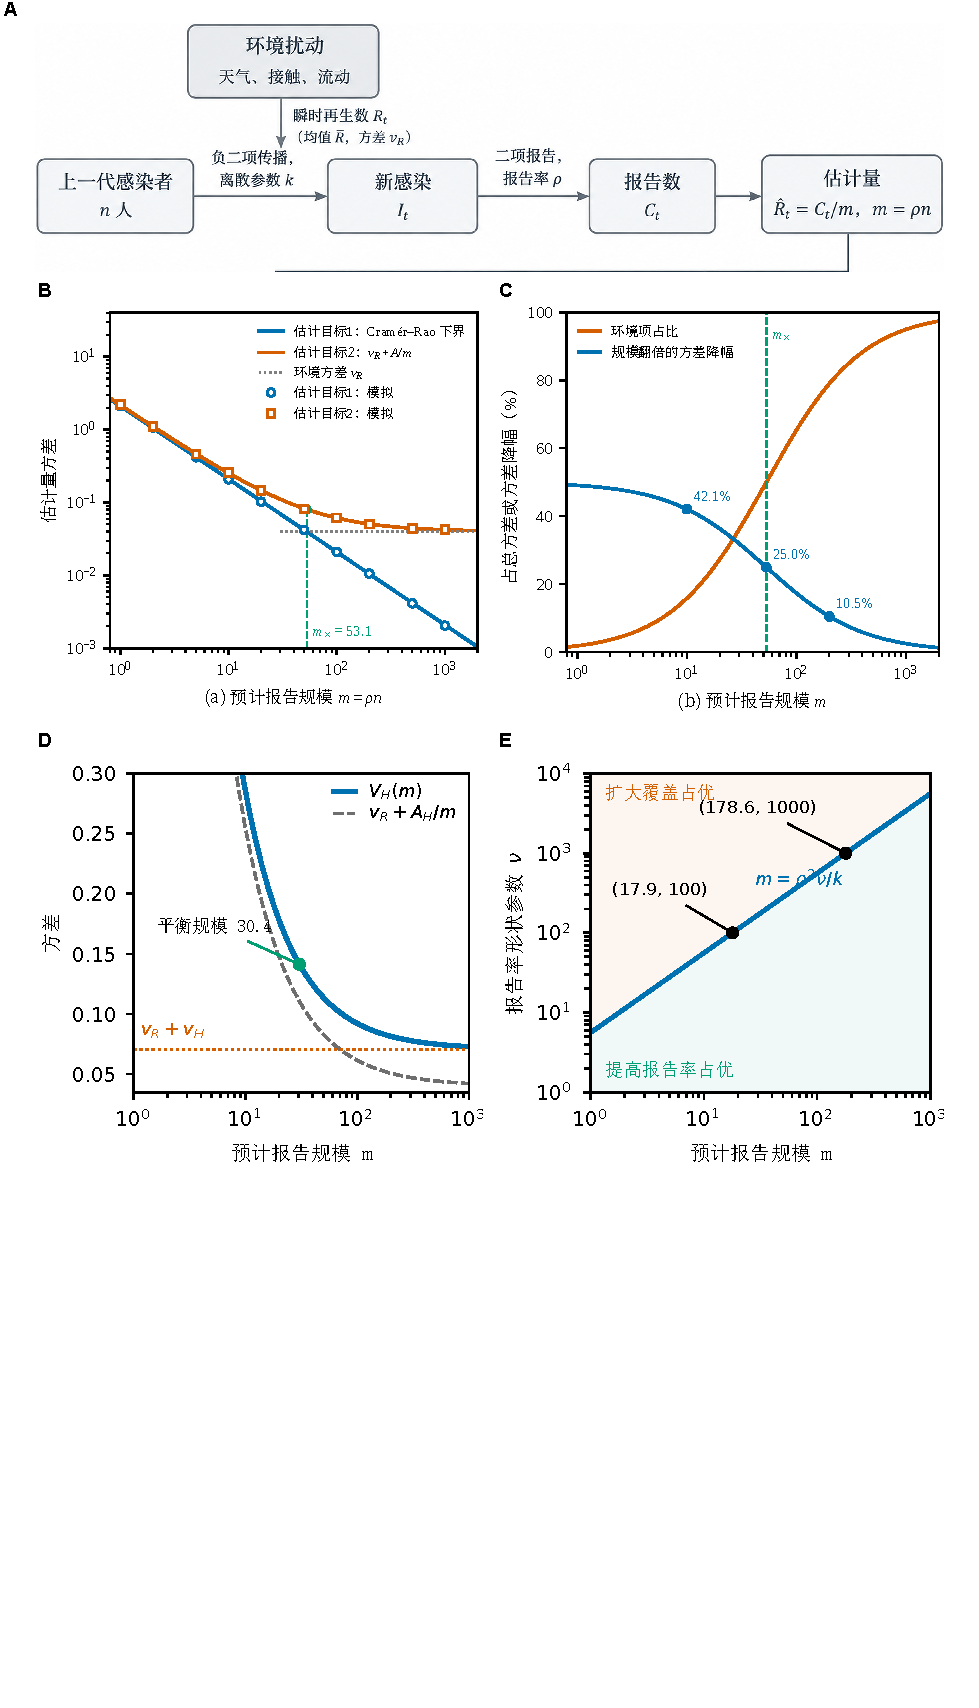
\includegraphics[width=0.98\textwidth]{figures/fig_main1.pdf}
  \caption{Model structure and theoretical variance decomposition. (A) Transmission and observation process: environmental disturbances determine the instantaneous reproduction number $R_t$; $n$ primary cases generate secondary infections $I_t$ via negative-binomial branching; infections undergo binomial thinning with probability $\rho$ into reported counts $C_t$; bottom row contrasts Target 1 ($R_t$) and Target 2 ($\bar{R}$). (B) Variance of the natural estimator $\widehat{R}_t = C_t/m$ as a function of expected reporting scale $m$, evaluated at baseline parameters ($\bar{R}=1.15, v_R=0.04, k=0.35, \rho=0.25$; $A=2.1232, m_\times=53.1$ cases); hollow circles denote 20,000 Monte Carlo replications; green dashed line marks the variance balance scale $m_\times$. (C) Proportion of environmental variance in total error and proportional variance reduction from scale doubling as a function of $m$; dotted markers highlight reductions of 42.1\%, 25.0\%, and 10.5\% at $m=10, 53.1, 200$. (D) Variance curve under reporting heterogeneity ($\tau=0.15$), where the balance scale contracts from 53.1 to 30.4 cases; dotted horizontal line denotes the asymptotic floor $v_R+v_H$. (E) Ranking reversal boundary between raising reporting completeness and expanding population coverage under binomial reporting volatility.}
  \label{fig:variance}
\end{figure}

\section{Results}
\label{sec:results}

\subsection{Diminishing returns from case volume for the mean reproduction number}
\label{sec:res-theory}

\begin{figure}[t]
  \centering
  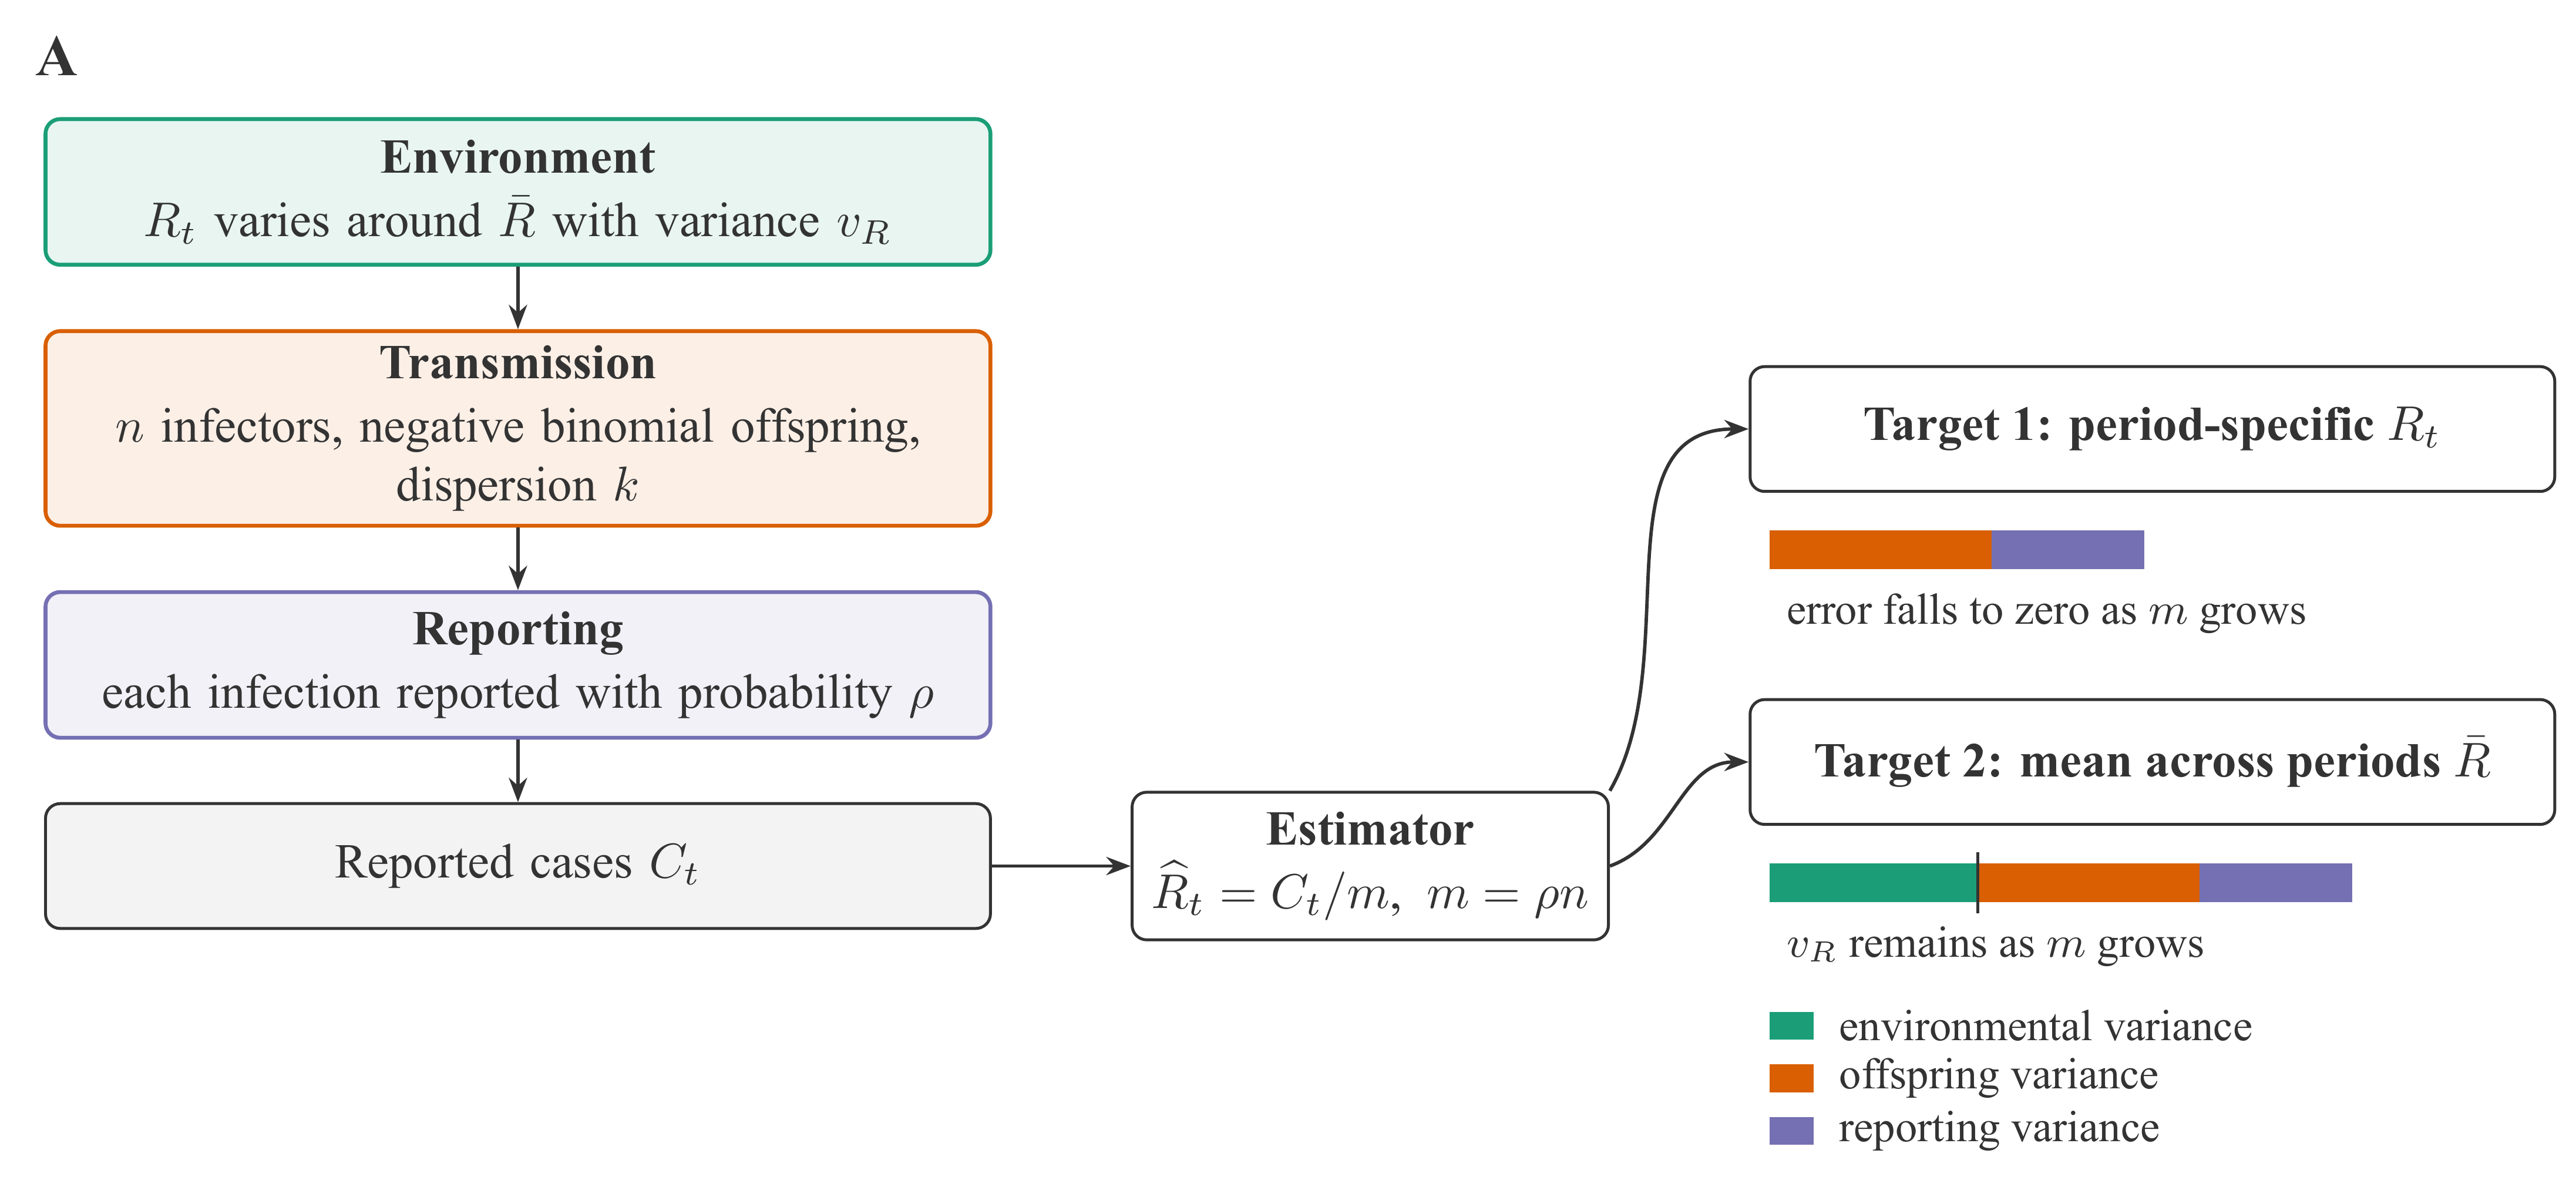
\includegraphics[width=0.86\linewidth]{figures/fig_01_schematic.png}\\[2pt]
  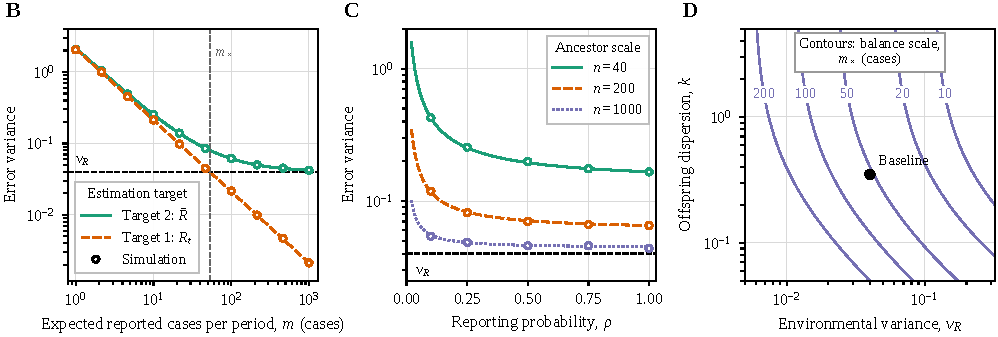
\includegraphics[width=\linewidth]{figures/fig_01_theory.pdf}
  \caption{Contributions of environmental, offspring and reporting variation to the error of the scaled estimator of the reproduction number. (A) Schematic of the two estimation targets, the period-specific value and the mean across periods, for the estimator that divides reported cases by expected case volume; colours mark the environmental, offspring and reporting sources of error. (B) Error variance against expected reported cases per period for the mean across periods and for the period-specific value; lines are closed forms, circles are Monte Carlo estimates with 95\% intervals, and dashed lines mark the environmental variance $v_R$ and the balance scale. (C) Error variance against reporting probability for three fixed numbers of primary cases; the value at full reporting is the residual offspring term. (D) Contours of the balance scale over environmental variance and offspring dispersion, with the baseline parameter set marked.}
  \label{fig:theory}
\end{figure}

Under the baseline parameters ($\Rbar=1.15$, $v_R=0.04$, $k=0.35$, $\rho=0.25$; see Materials and methods), the sampling coefficient was $A=2.1232$ and the balance scale was $\mx=53.1$ reported cases per period (Fig.~\ref{fig:theory}B). Error variance for the period-specific value fell in proportion to $1/m$ over the whole range, whereas error variance for the mean levelled off at $v_R$. Doubling the case volume reduced error variance for the mean by 42.1\% at $m=10$, by 25.0\% at $m=\mx$ and by 10.5\% at $m=200$. Monte Carlo estimates from 20000 replications per point differed from Eq.~(\ref{eq:var-average}) by at most 4.0\%.

Raising reporting probability at fixed coverage did not reduce error variance to $v_R$ (Fig.~\ref{fig:theory}C). At full reporting the residual variance was 0.166 with 40 primary cases, 0.0652 with 200 and 0.0450 with 1000, against $v_R=0.04$. Near the baseline, a proportional increase in coverage reduced error variance 1.85 times as much as the same proportional increase in reporting probability. The balance scale was largest where environmental variance was small and offspring were strongly overdispersed (Fig.~\ref{fig:theory}D).

\begin{figure}[t]
  \centering
  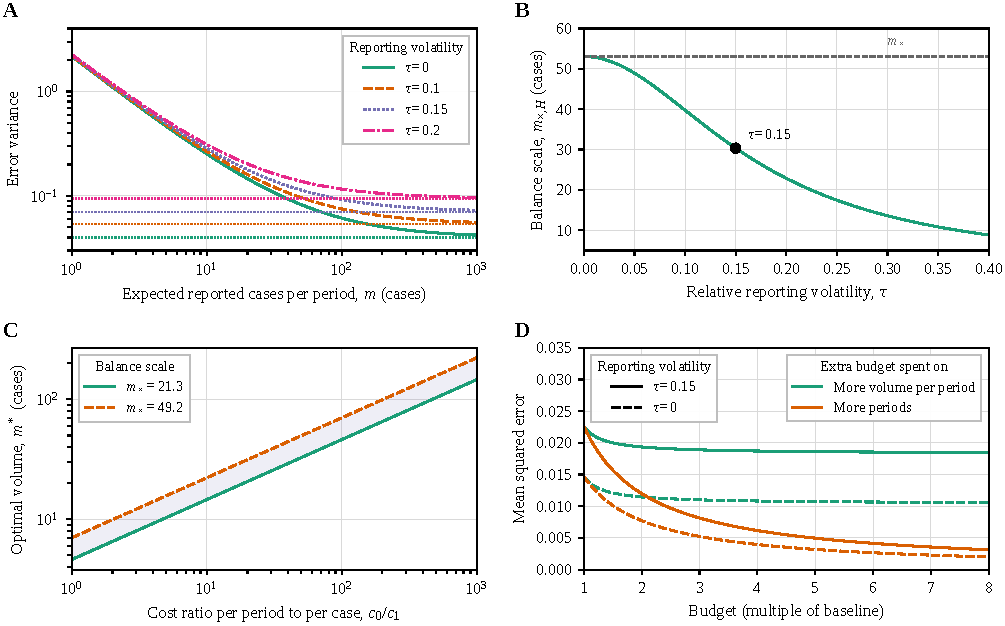
\includegraphics[width=0.92\linewidth]{figures/fig_02_heterogeneity_budget.pdf}
  \caption{Reporting heterogeneity and the allocation of a fixed surveillance budget. (A) Error variance against expected reported cases per period for four levels of relative reporting volatility; dotted lines mark the corresponding limits as case volume grows, set by environmental plus reporting variance. (B) Generalised balance scale against relative reporting volatility; the dashed line is the balance scale without reporting volatility, and the dot marks the volatility used in panel D. (C) Optimal number of reported cases per period against the price ratio $c_0/c_1$, for the two ends of the uncorrected scenario range of the balance scale, 21.3 and 49.2 cases per generation (labelled $m_\times$ in the panel); the band spans the range between them. (D) Mean squared error of the estimator of the mean reproduction number against total budget, when additional budget buys either more cases per period or more periods, with autocorrelated environmental and reporting variation, under baseline (solid) and standardised (dashed) reporting.}
  \label{fig:budget}
\end{figure}

A relative reporting volatility of $\tau=0.15$ added $v_H=0.0307$ to the limiting variance and reduced the balance scale from 53.1 to 30.4 cases (Fig.~\ref{fig:budget}A, B). The scenario parameters for influenza admissions give uncorrected balance scales of 21.3 to 49.2 cases per generation (Section~\ref{sec:meth-loss}); Section~\ref{sec:res-empirical} reports the latent value implied by the data. Over this range, the optimal case volume $m^*$ of Eq.~(\ref{eq:optimal-m}) was 14.6 to 22.2 cases per period for $c_0/c_1=10$ and 46.2 to 70.1 cases for $c_0/c_1=100$ (Fig.~\ref{fig:budget}C). In a hypothetical example with ten periods of 50 cases, autocorrelated environment ($\phi=0.5$) and reporting (with relative reporting perturbation autocorrelation $\psi=0.5$, see Appendix~\ref{app:random-denominator}) and $\tau=0.15$, the mean squared error of the mean was $22.57\times10^{-3}$, of which $10.40\times10^{-3}$ was environmental, $7.88\times10^{-3}$ reporting and $4.29\times10^{-3}$ sampling (Table~\ref{tab:s7}). A tenfold increase in case volume reduced it to $18.71\times10^{-3}$, whereas standardising reporting reduced it to $14.65\times10^{-3}$ and four times as many periods to $6.17\times10^{-3}$. At twice the baseline budget, spending the increment on cases gave $19.35\times10^{-3}$ and spending it on periods gave $11.98\times10^{-3}$ (Fig.~\ref{fig:budget}D).

\subsection{Calibration of apparent weekly statistics by simulation}
\label{sec:res-sim}

\begin{figure}[t]
  \centering
  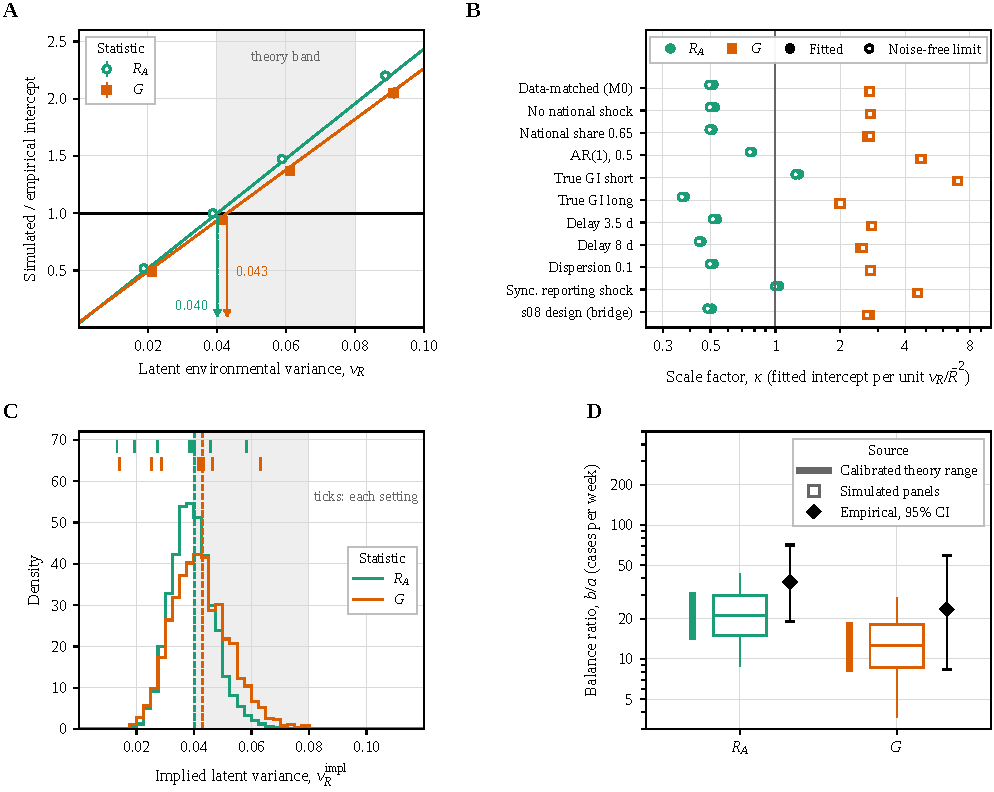
\includegraphics[width=\linewidth]{figures/fig_03_sim_inversion.pdf}
  \caption{Simulation-based inversion from apparent statistics to latent dynamics. (A) Calibration lines from 200 simulated panels per cell that reproduce the observed seasons, window lengths, state sizes, national week shocks and reporting delay. Fitted intercepts are scaled by the empirical intercept. Dashed drop lines mark where each line meets the data, giving the implied latent variance $v_R$. (B) Scale factor $\kappa$ linking the fitted intercept to $v_R/\Rbar^2$ for each simulation setting. Filled markers are fitted values and open markers the noise-free limit. (C) Distribution of the implied $v_R$ under the data-matched setting. Uncertainty combines the two-way bootstrap of the data with Monte Carlo error of the calibration. Top ticks show the point values of the other settings. (D) Simulated per-panel $b/a$ and the calibrated theoretical range, against empirical estimates with 95\% intervals. Grey bands mark $v_R=0.04$--0.08.}
  \label{fig:inversion}
\end{figure}

The empirical statistics are apparent quantities. The weighted growth ratio $G$ compounds more than one generation of growth into a week, and the renewal-type ratio $R_A$ maps weekly growth back to the generation scale through an assumed generation interval (Section~\ref{sec:meth-stats}). Their intercepts therefore need a calibration before they can be compared with $v_R$. We built this calibration in a simulation that reproduces the observed panel (Section~\ref{sec:meth-inversion}). It keeps the four seasons, the rule-window lengths and the initial admissions of each state, and adds a national week shock that carries 45\% of $v_R$ and the delay from infection to admission. We simulated 200 panels at each of four values of $v_R$. The mean fitted intercept rose linearly with $v_R$ for both statistics (Fig.~\ref{fig:inversion}A), and no cell mean departed from the fitted line by more than 0.60 Monte Carlo standard errors.

Expressed as a scale factor on $v_R/\Rbar^2$, the fitted intercept was $\kappa=0.516$ for $R_A$ and 2.729 for $G$, close to the noise-free limits of 0.493 and 2.745 (Fig.~\ref{fig:inversion}B). A simpler design with 500 independent states and six observation weeks gave noise-free limits of 0.485 and 2.698, in line with the medians of 0.484 and 2.68 over the 17 scenarios of the first simulation. The data-matched panels also reproduced the dependence structure of the data. The intraclass correlation of weekly losses within calendar weeks was 0.258 for $R_A$ and 0.310 for $G$ in simulation, against 0.253 and 0.310 in the data, and the national-week share of the simulated $R_A$ intercept was 0.43, against 0.41 observed. Across settings that changed one ingredient at a time, $\kappa$ for $R_A$ moved most with the true generation interval (1.287 for a mean of 2.2 days and 0.380 for 4.3 days, with the statistic still computed at 3.6 days), with autocorrelation of transmission between weeks (0.780 at $\phi=0.5$) and with a synchronous shock to reported counts (1.041). It changed little with the national share of the shock, the admission delay or the offspring dispersion (0.454 to 0.535; Table~\ref{tab:s8}).

\subsection{Empirical intercepts and the implied environmental variance}
\label{sec:res-empirical}

\begin{figure}[t]
  \centering
  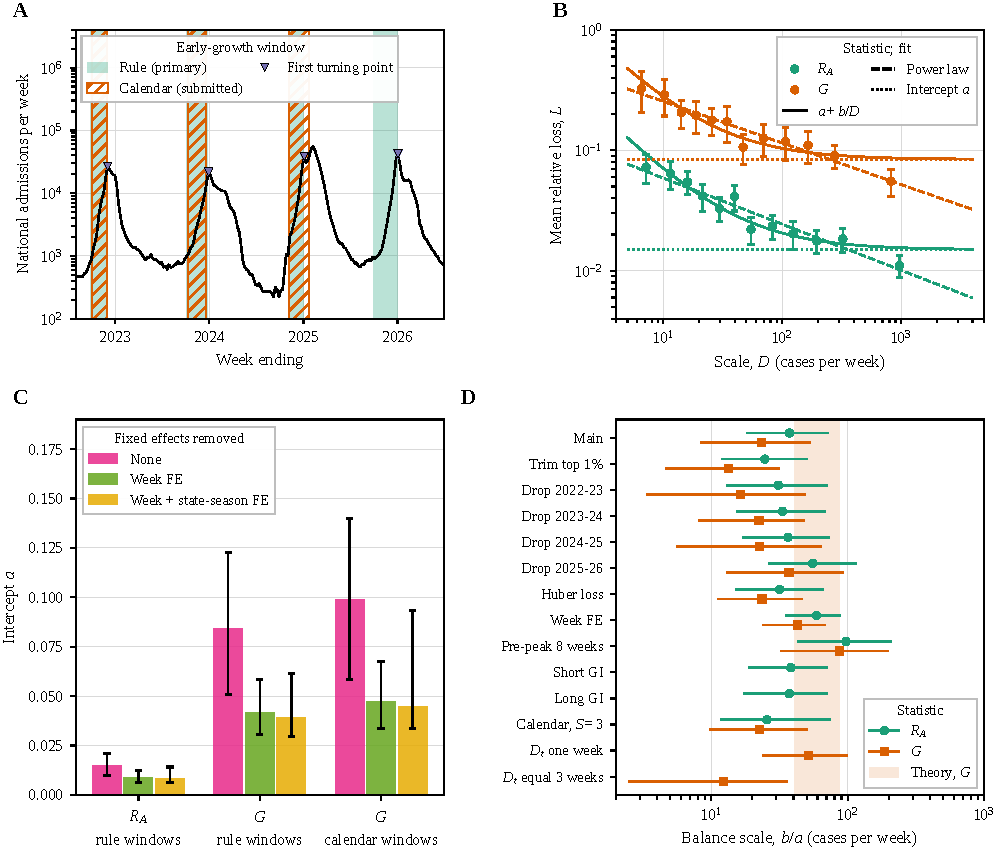
\includegraphics[width=0.86\linewidth]{figures/fig_04_empirical_loss.pdf}
  \caption{Relative loss of two apparent weekly statistics in influenza hospital admissions. (A) National weekly admissions on a logarithmic scale; shading marks the rule-based early-growth windows of the primary analysis, hatching marks the calendar windows of the earlier analysis, and triangles mark the first national turning point of each season. (B) Binned mean relative loss against reporting scale for the renewal-type ratio and the weighted growth ratio, with the fitted affine curve, a power law without intercept used for comparison and the fitted intercept; bin error bars ignore clustering. (C) Intercept before adjustment, after removing national-week effects and after also removing state-season effects, with two-way bootstrap intervals. (D) Ratio of slope to intercept under sensitivity variants; the band is the uncalibrated theoretical range for the growth ratio with the denominator correction, and Fig.~\ref{fig:inversion}D gives the calibrated range.}
  \label{fig:floor}
\end{figure}

In the rule-defined early-growth windows of four seasons, 1748 state-weeks in 42 calendar weeks gave a renewal-type ratio intercept of $a=0.0150$ (95\% CI 0.0100 to 0.0208), slope $b=0.560$ (95\% CI 0.367 to 0.769) and $b/a=37.4$ (95\% CI 19.1 to 71.0) (Fig.~\ref{fig:floor}B; Table~\ref{tab:s1}). The weighted growth ratio in the same windows gave $a=0.0840$ (95\% CI 0.0498 to 0.1248) and $b/a=23.5$ (95\% CI 8.4 to 59.7) from 1756 state-weeks. The eight additional state-weeks have a reporting scale $D_t$ of at least five but fewer than five admissions in the current week, which $R_A$ requires because its scale is the single-week count. In the three calendar windows of the earlier analysis, the growth ratio gave $a=0.0991$ (95\% CI 0.0569 to 0.1382) and $b/a=22.6$ (95\% CI 9.0 to 52.2). Within the affine model, all bootstrap replicates gave a positive intercept for both rule-window specifications, as did 99.95\% for the calendar windows. The bootstrap standard deviation of $a$ was 1.95 to 4.68 times that obtained by resampling states only.

The ratio $b/a$ varied across specifications by a factor of 3.9 for $R_A$, from 24.7 after trimming the most influential 1\% of losses to 97.1 in peak weeks, and by a factor of 7.1 for $G$, from 12.2 with equal denominator weights to 86.8 in peak weeks (Fig.~\ref{fig:floor}D). Generation interval variants changed it by less than 3\% for $R_A$. Over the observed range of scales, a power law without an intercept fitted the binned losses about as well as the affine form (bootstrap $p=0.114$ for $R_A$, 0.438 and 0.418 for $G$; Table~\ref{tab:s2}). Cross-validation by state and by season did not consistently favour the affine form, and a power analysis found no fraction of the estimated intercept detectable with 80\% power (Table~\ref{tab:s2}). The data therefore do not distinguish a positive floor from a loss that keeps declining as a power of the reporting scale. The affine form was retained because its parameters correspond to Proposition~\ref{prop:average} and enter the calibration directly. Under the power law no balance scale exists, so the intercept, the apparent balance ratio and the quantities derived from them below are conditional on the affine form.

Mapping each empirical intercept through its calibration line gave an implied latent variance of $v_R^{\mathrm{impl}}=0.040$ (95\% CI 0.026 to 0.056) for $R_A$ and 0.043 (95\% CI 0.025 to 0.064) for $G$ (Fig.~\ref{fig:inversion}A, C). Bootstrap variation in the empirical intercept accounted for nearly all of this width, since the interval from calibration error alone was 0.0397 to 0.0406 for $R_A$. The scale factors of the two statistics differ by a factor of 5.3. Their implied variances differed by $-0.003$ (95\% CI $-0.012$ to 0.005), a ratio of 0.93 (95\% CI 0.78 to 1.18). The 90\% interval of this ratio, 0.81 to 1.13, lies within 0.80 to 1.25, so two one-sided tests at the 5\% level declare the two estimates equivalent within a margin of 20\%. This concordance serves as a model-consistency check under the reference simulator, although it has limited discriminating power across the wider sensitivity space where the two statistics also produced overlapping intervals in nine of the ten simulated settings (Table~\ref{tab:s8}). Both point values lie at the lower edge of the band of 0.04 to 0.08 used in the scenario calculations, and both intervals extend below it. On the latent scale, Proposition~\ref{prop:average} at the simulator values ($\Rbar=1.18$, $\rho=\rho_h=0.01$, $k=0.35$) gives a balance scale of 30.3 admissions per generation (95\% CI 21.7 to 46.3) for $R_A$, or about 59 per week at 1.94 generations per week. The apparent ratio of 37.4 is defined on the scale of $R_A$ and does not estimate this latent quantity directly. The latent scale moves with the implied variance; at the value of 0.026 obtained with a true mean generation interval of 2.9 days (below), the same formula gives about 47 admissions per generation, or roughly 110 per week.

Across ten settings, $v_R^{\mathrm{impl}}$ ranged from 0.013 to 0.063 (Fig.~\ref{fig:inversion}C; Table~\ref{tab:s8}). The true generation interval had the largest effect, giving 0.013 and 0.014 when it was shorter than the 3.6 days assumed by the statistic and 0.058 and 0.063 when it was longer. The interval of the primary estimate does not include this source of variation. The 95\% interval of the difference between the two statistics contained zero in nine of the ten settings; this non-rejection is the sense of agreement used in Table~\ref{tab:s8}. The exception replaced the transmission shock by a synchronous multiplicative shock to reported counts, which gave 0.019 for $R_A$ and 0.029 for $G$ (ratio 0.67; 95\% CI 0.39 to 0.90).

Three classes of sensitivity analyses examined the assumptions of the inversion (Table~\ref{tab:s10}). The lag-1 autocorrelation of deviations from state-season means was $-0.095$ (95\% CI $-0.168$ to $-0.019$) for $R_A$ and 0.123 (95\% CI 0.039 to 0.201) for $G$. Both statistics are autocorrelated by construction even when weekly shocks are independent; simulated panels with independent shocks gave means of $-0.074$ and 0.114, which placed the data at the 31st and 62nd percentiles. With a first-order coefficient of 0.25 the data fell at the 3rd and 10th percentiles, and with 0.5 below all simulated panels. The mean household serial interval of seasonal influenza has been estimated at 3.6 days (95\% CI 2.9 to 4.3) \citep{cowling2009estimation}, and direct estimates of the mean generation interval lie near the lower end of this interval \citep{chan2025estimating}. With a true mean generation interval of 2.9 days, the implied variance was 0.026 (95\% CI 0.017 to 0.036) for $R_A$ and 0.027 (95\% CI 0.016 to 0.040) for $G$; with 4.3 days it was 0.058 and 0.063. The autocorrelation of the data sat at the 2.5th and 9th percentiles of panels simulated with 2.9 days and at the 80th and 92nd percentiles with 4.3 days. This state-level check therefore does not favour the shorter interval, although it leaves the series of national-week means untested (Section~\ref{sec:meth-inversion}). The shorter interval did reproduce the empirical $b/a$. At $v_R=0.02$, the simulated value nearest its implied variance, the data sat at the 52.5th and 58th percentiles of the simulated $b/a$. Overdispersed weekly admissions with a variance-to-mean ratio of 1.5 or 2.0 kept the implied variance between 0.039 and 0.045. They raised the simulated $b/a$ at $v_R=0.04$ from 28.0 to 68.0 and 81.0 for $R_A$, and from 16.2 to 40.2 and 48.4 for $G$. These settings also gave lag-1 autocorrelations below the data for both statistics, so the data were more compatible with overdispersion smaller than a variance-to-mean ratio of 1.5 under this simulator.

On the scale of each statistic, the calibrated theory gave $b/a$ of 13.9 to 31.1 for $R_A$ and 8.0 to 18.8 for $G$ over eight combinations of $v_R\in\{0.04,0.08\}$, $k\in\{0.2,0.5\}$ and admission probability $\rho_h\in\{0.0056,0.021\}$ (Fig.~\ref{fig:inversion}D). The empirical point estimates of 37.4 and 23.5 lie above these ranges, and their 95\% intervals overlap them. Ratios from single simulated panels varied widely; 95\% of them lay between 8.8 and 42.7 for $R_A$ and between 3.6 and 28.6 for $G$, and the empirical values fall at the 93rd and 91st percentiles of these distributions. Overdispersed admissions and a shorter generation interval can each raise the simulated ratio to the empirical values (Table~\ref{tab:s10}). A further explanation lies outside the simulator, which gives every state the same intercept. If larger states average environmental variation over more local epidemics (Eq.~(\ref{eq:pooling})), part of the cross-sectional slope reflects spatial aggregation and the empirical $b/a$ is inflated.

\subsection{Multiscale decomposition of surveillance uncertainty}
\label{sec:res-multiscale}

The intercept contains a component shared by all states in a calendar week and a component specific to states (Fig.~\ref{fig:floor}C; Table~\ref{tab:s2}). Removing national-week effects reduced $a$ by 41\% (95\% CI 12 to 59) for $R_A$ and by 51\% (95\% CI 21 to 67) for $G$ in rule windows, and by 52\% for $G$ in calendar windows. Removing state-season effects as well changed the intercept little; for $R_A$ it was 0.0083 (95\% CI 0.0064 to 0.0141) after both adjustments, and the interval for the state-season component included zero in every specification. The intraclass correlation of the loss within calendar weeks was 0.253 for $R_A$ and 0.310 for $G$. The bootstrap reflected the same structure. Resampling weeks alone gave a standard deviation of $\hat{a}$ of 0.0021 for $R_A$ and 0.0158 for $G$, 1.46 and 1.87 times the values from resampling states alone, and two-way resampling gave 0.0028 and 0.0193.

The national-week component enters the loss of every state in the same week. More admissions in one state reduce only that state's count term, and averaging over states reduces only the state-specific term, so neither removes the shared component; only further weeks average it out. Pooling the mean weekly deviation over $J$ randomly chosen states reduced its variance to 0.39, 0.31 and 0.25 of the single-state value for $R_A$ at $J=5$, 10 and 51, and to 0.43, 0.36 and 0.31 for $G$ (Fig.~\ref{fig:design}C). These values approach the national-week component, which is 0.23 of single-state variance for $R_A$ and 0.29 for $G$, and come within 10\% of it at $J=33$ and $J=25$ respectively, as Eq.~(\ref{eq:pooling}) predicts for partly synchronised variation.

\subsection{Mandatory and voluntary reporting regimes}
\label{sec:res-reporting}

\begin{figure}[t]
  \centering
  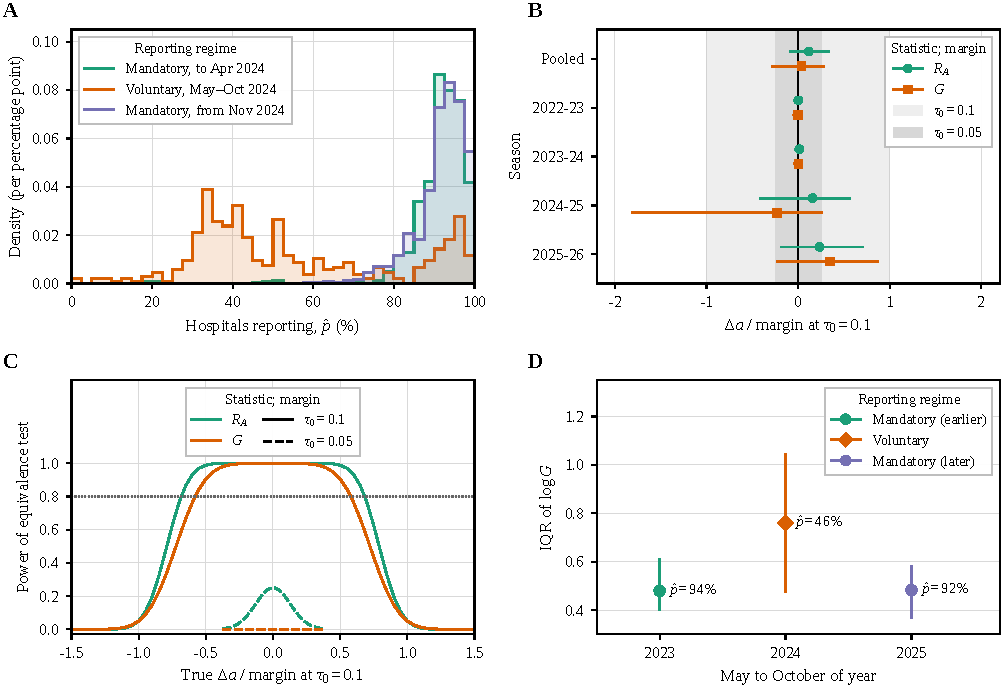
\includegraphics[width=0.86\linewidth]{figures/fig_05_reporting.pdf}
  \caption{Reporting completeness and the empirical intercept. (A) Distribution of the share of hospitals reporting influenza admissions under the three reporting regimes. (B) Change in the intercept when the statistic is adjusted for reporting coverage, pooled and by season, with 90\% paired bootstrap intervals. Each statistic is expressed relative to its own equivalence margin, and shaded bands show the margins implied by two thresholds of reporting volatility. (C) Power of the two one-sided equivalence test against the true change, for both statistics and both margins, with a conventional power reference. (D) Interquartile range of the logarithm of the growth ratio over May to October in three calendar years; the year with voluntary reporting is highlighted, and labels give median reporting completeness.}
  \label{fig:reporting}
\end{figure}

Among state-weeks with a reporting scale of at least five, the median share of hospitals reporting was 92.3\% in the first mandatory period, 45.7\% under voluntary reporting and 92.9\% after mandatory reporting resumed (Fig.~\ref{fig:reporting}A). In the rule windows the median was 93.7\%, and 79.8\% of state-weeks had at least 90\% of hospitals reporting. Within these windows, adjusting each statistic for the reporting share changed the intercept of $R_A$ by $\Delta a=0.29\times10^{-3}$ (90\% CI $-0.22\times10^{-3}$ to $0.85\times10^{-3}$) and that of $G$ by $0.37\times10^{-3}$ (90\% CI $-2.83\times10^{-3}$ to $2.81\times10^{-3}$) (Fig.~\ref{fig:reporting}B; Table~\ref{tab:s3}). Both changes were equivalent to zero within margins set at a relative reporting volatility of $\tau_0=0.10$. These margins equal 17\% (95\% CI 12 to 25) of the intercept of $R_A$ and 12\% (95\% CI 8 to 20) of that of $G$, and they depend on the sample mean of each statistic through Eq.~(\ref{eq:tost}). The measured change was 2.0\% of the intercept for $R_A$ (95\% CI $-2.4$ to 6.1; one-sided 95\% upper bound 5.3\%, the 95th percentile of the bootstrap distribution of the share) and 0.4\% for $G$ (95\% CI $-4.4$ to 4.0; upper bound 3.5\%), and all four seasons for $R_A$ and three of four for $G$ were equivalent individually. At $\tau_0=0.05$, with margins of about 4\% and 3\% of the intercepts, neither change was equivalent, and the power of the test at a true change of zero was 0.25 for $R_A$ and 0 for $G$ (Fig.~\ref{fig:reporting}C). Because most state-weeks in the windows had nearly complete participation, these tests bound the effect of small departures from full participation and do not extend to low participation.

The voluntary period gave the only contrast in which reporting completeness was low. Over May to October, the interquartile range of $\log G$ was 0.759 in 2024 under voluntary reporting, against 0.479 in 2023 and 0.483 in 2025 (Fig.~\ref{fig:reporting}D; Table~\ref{tab:s4}). The ratio of 2024 to 2023 was 1.58 (95\% CI 0.95 to 2.23) and that of 2024 to 2025 was 1.57 (95\% CI 0.95 to 2.39), whereas the placebo ratio of 2025 to 2023 was 1.01 (95\% CI 0.72 to 1.25). Median reporting scales in these months were similar (15.6, 16.6 and 16.2 admissions), and matching state-weeks on reporting scale gave ratios of 1.68 and 1.58. Matching on calendar month gave a median ratio of 1.33, with the ratio above one in nine of twelve month-by-year comparisons. COVID-19 admissions showed ratios of 1.62 against 2023 and 1.18 against 2025, and RSV admissions a ratio of 1.36 against 2025. All of these comparisons use the same off-season of 2024 and are not independent replications. In 44 states with laboratory data, laboratory $R_A$ correlated with hospital $R_A$ at $r=0.31$ and shared 0.230 (95\% CI 0.043 to 0.418) of the hospital intercept.

\subsection{Diminishing returns and surveillance design}
\label{sec:res-design}

\begin{figure}[t]
  \centering
  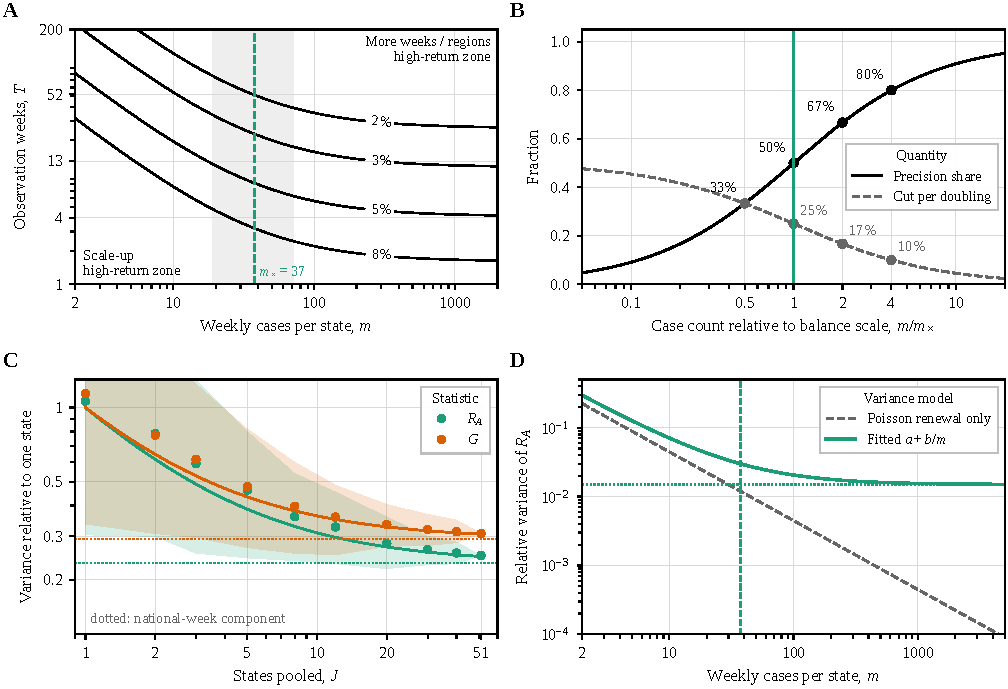
\includegraphics[width=\linewidth]{figures/fig_06_design_nomogram.pdf}
  \caption{Surveillance design nomogram. (A) Observation weeks needed for the relative standard error of a single state's mean renewal ratio $R_A$ to reach 2--8\%, by weekly admissions $m$, on the scale of the statistic and ignoring autocorrelation within states. The dashed line marks the apparent balance ratio $b/a$ of $R_A$ (labelled $m_\times$ in the legacy panel asset), and the grey band its 95\% interval. To its left, added cases give most of the gain. To its right, contours flatten and added weeks or regions give most of the gain. (B) Share of attainable precision, $m/(m+\mx)$, and the variance reduction from one doubling of $m$. (C) Variance of the mean weekly deviation pooled over $J$ states, relative to one state, for $R_A$ and the growth ratio $G$. Points and bands come from random state subsets; dotted lines show the national-week component. (D) Relative variance of $R_A$ under the Poisson renewal variance alone and under the fitted $a+b/m$.}
  \label{fig:design}
\end{figure}

Under $V(m)=a+b/m$, the share of the precision attainable at unlimited case volume is $m/(m+\mx)$, and one doubling of $m$ reduces variance by the fraction $\mx/[2(m+\mx)]$ (Proposition~\ref{prop:average}). The share is 33\%, 50\%, 67\% and 80\% at $m=0.5$, 1, 2 and 4 times $\mx$, a doubling from these points cuts variance by 33\%, 25\%, 17\% and 10\%, and 90\% of attainable precision requires $m=9\mx$ (Fig.~\ref{fig:design}B). With the apparent balance ratios of 37.4 for $R_A$ and 23.5 for $G$, 55\% and 65\% of state-weeks in the rule windows lay above the ratio of the corresponding statistic. These shares refer to the apparent scale. The latent balance scale implied by the data, about 59 admissions per week (Section~\ref{sec:res-empirical}), is higher, so fewer state-weeks (approximately 43.5\%) lie above it on the latent per-generation scale, and a shorter generation interval would raise the latent scale further (roughly 110 per week at 2.9 days). For a single state, the number of observation weeks needed to reach a given relative standard error of mean $R_A$ fell steeply with admissions below $\mx$ and changed little above about $4\mx$ (Fig.~\ref{fig:design}A). Substituting the empirical apparent balance ratio $b/a$ into the allocation formula gives apparent-scale design analogues of the optimal case volume: $m^*=19.4$ (95\% CI 13.8 to 26.6) for $R_A$ and 15.3 for $G$ at $c_0/c_1=10$, and $m^*=61.2$ and 48.4 at $c_0/c_1=100$. Note that at $c_0/c_1=100$, the economic switching threshold $m^*=61.2$ exceeds the apparent balance ratio $37.4$, confirming that the condition for prioritising additional periods over cases per period is $m > m^*$, whereas the balance scale itself governs the onset of diminishing marginal returns.

The fitted variance departs from that of a Poisson renewal model, in which the error variance of the estimate is $\Rbar/m$ and has no term that persists as $m$ grows (Fig.~\ref{fig:design}D). On the apparent scale of $R_A$, the fitted slope ($b=0.560$) was 1.25 times the delta-method Poisson renewal slope $b_P = 0.446$ (computed as $\E[\kappa_A^2(1+C_t/C_{t+1})]$, which propagates Poisson count variance through the nonlinear renewal transformation), and the fitted variance was twice the Poisson variance at $m=22$ and ten times at $m=261$. On the latent scale of Proposition~\ref{prop:average}, with $v_R=0.040$, the corresponding values were $m=28$ and $m=262$.

Seasons limit any estimate of variation between seasons (Fig.~\ref{fig:seasons}). Season-specific intercepts of $R_A$ were 0.0137, 0.0062, 0.0127 and 0.0225, with a random-effects mean of 0.0125 (95\% CI 0.0022 to 0.0227) and $I^2=0.47$ (Table~\ref{tab:s5}). For $G$ the random-effects mean was 0.0619 (95\% CI 0.0066 to 0.1171) in rule windows and 0.0735 (95\% CI $-0.0558$ to 0.2028) in calendar windows. The relative standard error of any unbiased estimate of the between-season variance is at least 1.00 with three seasons and 0.82 with four (Corollary~\ref{cor:season}). Intercept ratios for alternative denominator weights showed $q_1<1<q_2$ for influenza, COVID-19 and RSV, for example $q_1=0.688$ and $q_2=1.539$ for influenza in calendar windows (Table~\ref{tab:s6}). Epidemic growth with reporting noise and no environmental variation gave ranges of 0.63 to 0.89 for $q_1$ and 1.13 to 1.58 for $q_2$ in calendar windows, so this ordering does not discriminate between mechanisms. Of 40 one-sided tests, 21 were significant before correction, 18 after Benjamini--Hochberg correction and 10 after Holm correction, all of them for influenza and none for departures from the null ranges.


\begin{figure}[!p]
  \centering
  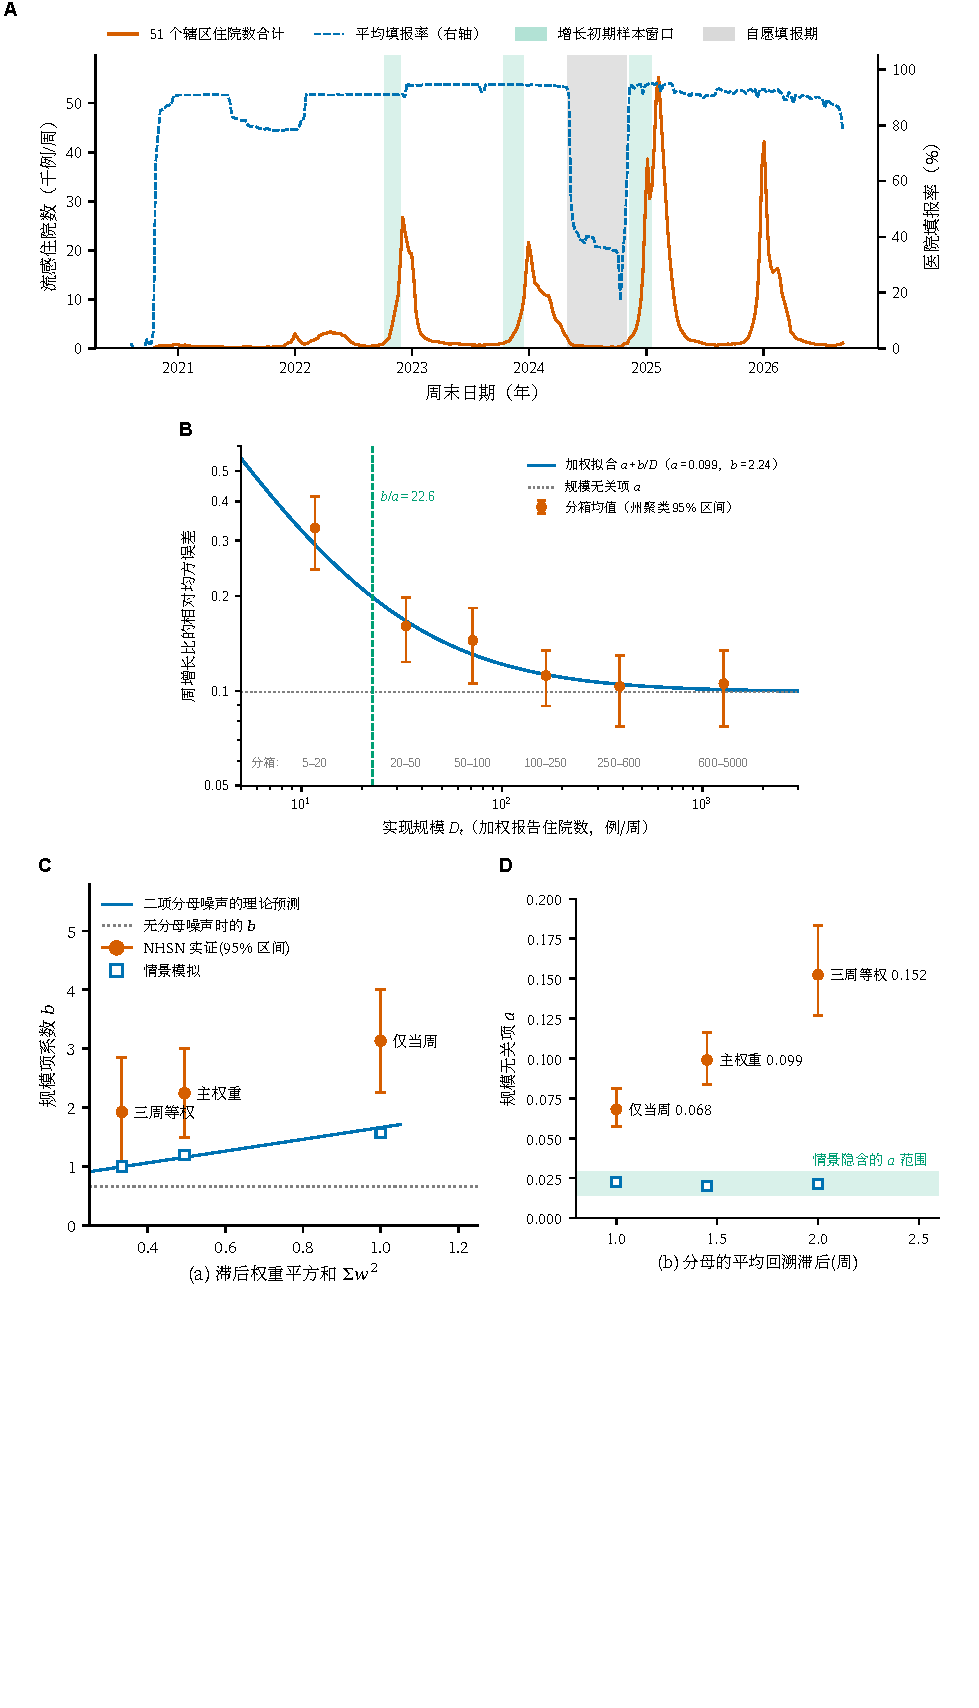
\includegraphics[width=0.92\textwidth]{figures/fig_main2.pdf}
  \caption{Scaling law and reporting signature in US influenza hospitalisation surveillance. (A) National weekly reported influenza hospitalisations and seasonal delineation (NHSN 2020--2026). (B) Binned mean squared loss of weekly hospitalisation growth against inverse sample scale $1/D_t$ in early epidemic phases, with FGLS affine fit $L = a + b/D_t$ (dashed curve); point area reflects state-week sample size. (C) Scaling slope coefficient $b$ versus sum of squared lag weights $\sum_s w_s^2$ across three weighting schemes; points with error bars represent NHSN estimates and 95\% CIs, squares denote scenario renewal simulations, solid line is the theoretical binomial denominator noise prediction, and dotted line indicates the noise-free denominator baseline. (D) Estimated intercept $a$ versus average denominator lookback lag, with scenario-implied intercept bounds shown in shaded grey.}
  \label{fig:case}
\end{figure}

\begin{figure}[!p]
  \centering
  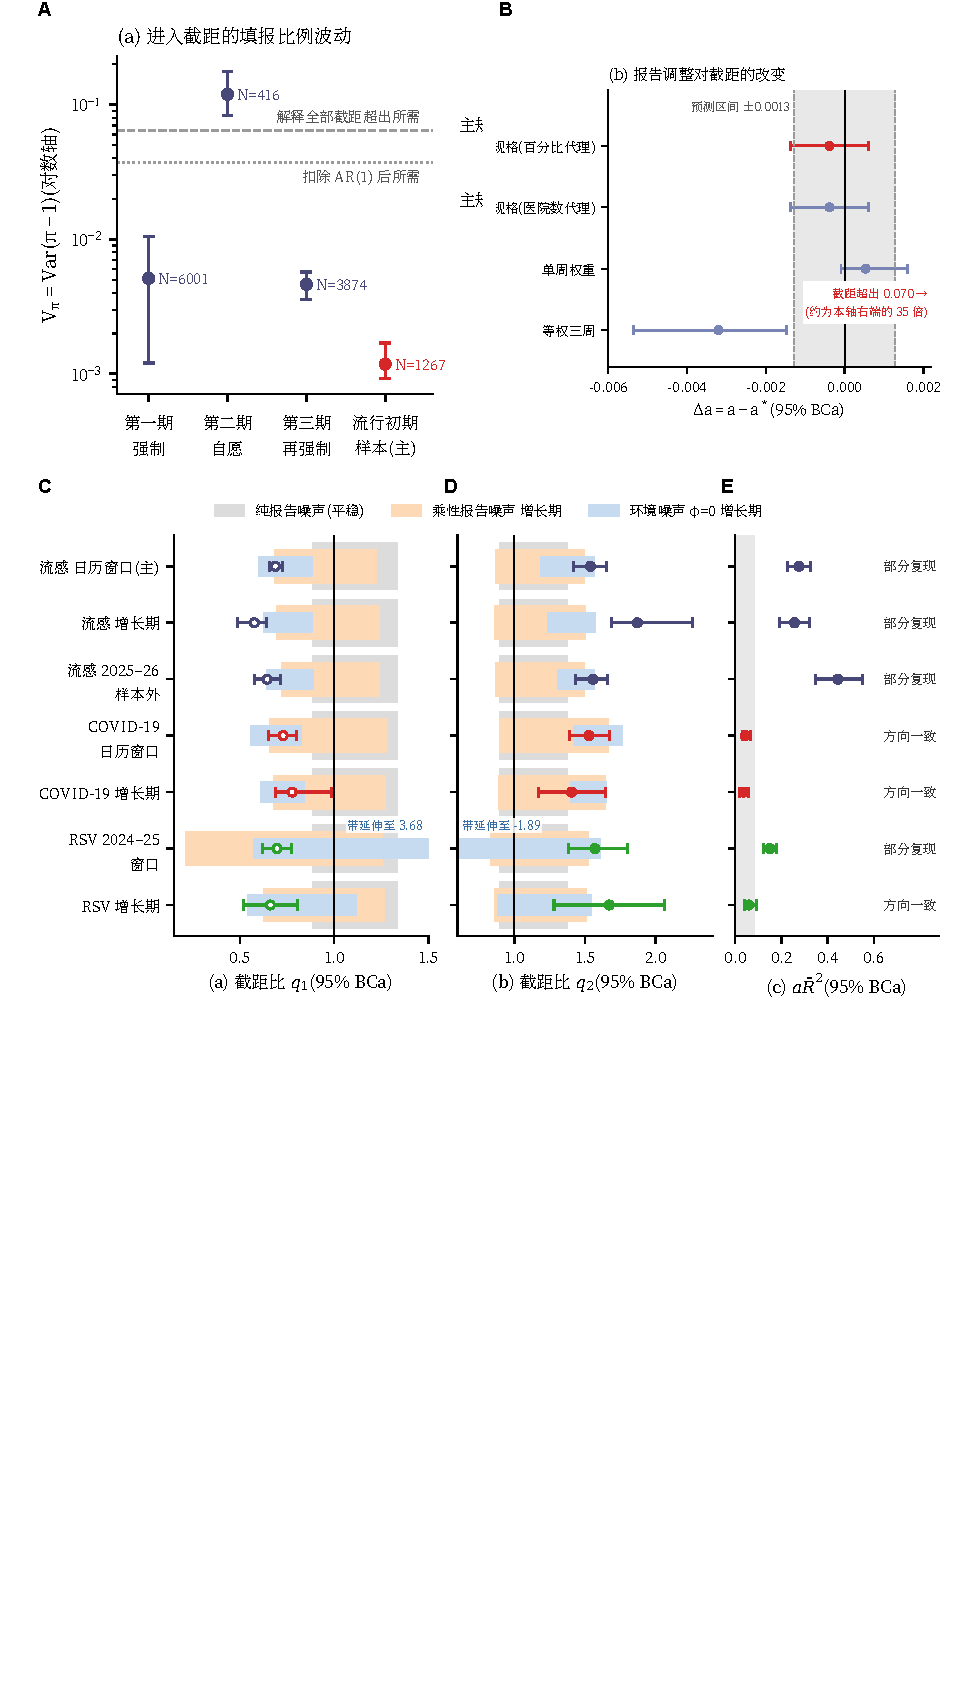
\includegraphics[width=0.92\textwidth]{figures/fig_main3.pdf}
  \caption{Reporting adjustment and cross-pathogen replication. (A) Volatility of hospital reporting completeness ratios $V_\pi$ across three institutional reporting regimes and early-epidemic samples (logarithmic axis); horizontal reference lines indicate the reporting volatility required to explain the entire intercept excess or residual excess. (B) Difference in estimated intercept $\Delta a = a - a^*$ following hospital reporting adjustment across weighting vectors, with shaded band denoting pre-registered equivalence bounds ($\pm 0.0050$). (C) Empirical intercept ratios $q_1$ and (D) $q_2$ across seven pathogen-window combinations in NHSN; grey bands indicate analytical pure reporting noise bounds, and orange/blue bands represent simulated renewal null ranges. (E) Implied biological variance $a\bar{R}^2$ if intercepts were attributed entirely to environmental stochasticity, with right-hand labels denoting pre-registered replication classifications.}
  \label{fig:reporting-adj}
  \label{fig:pathogens}
\end{figure}

\begin{figure}[!p]
  \centering
  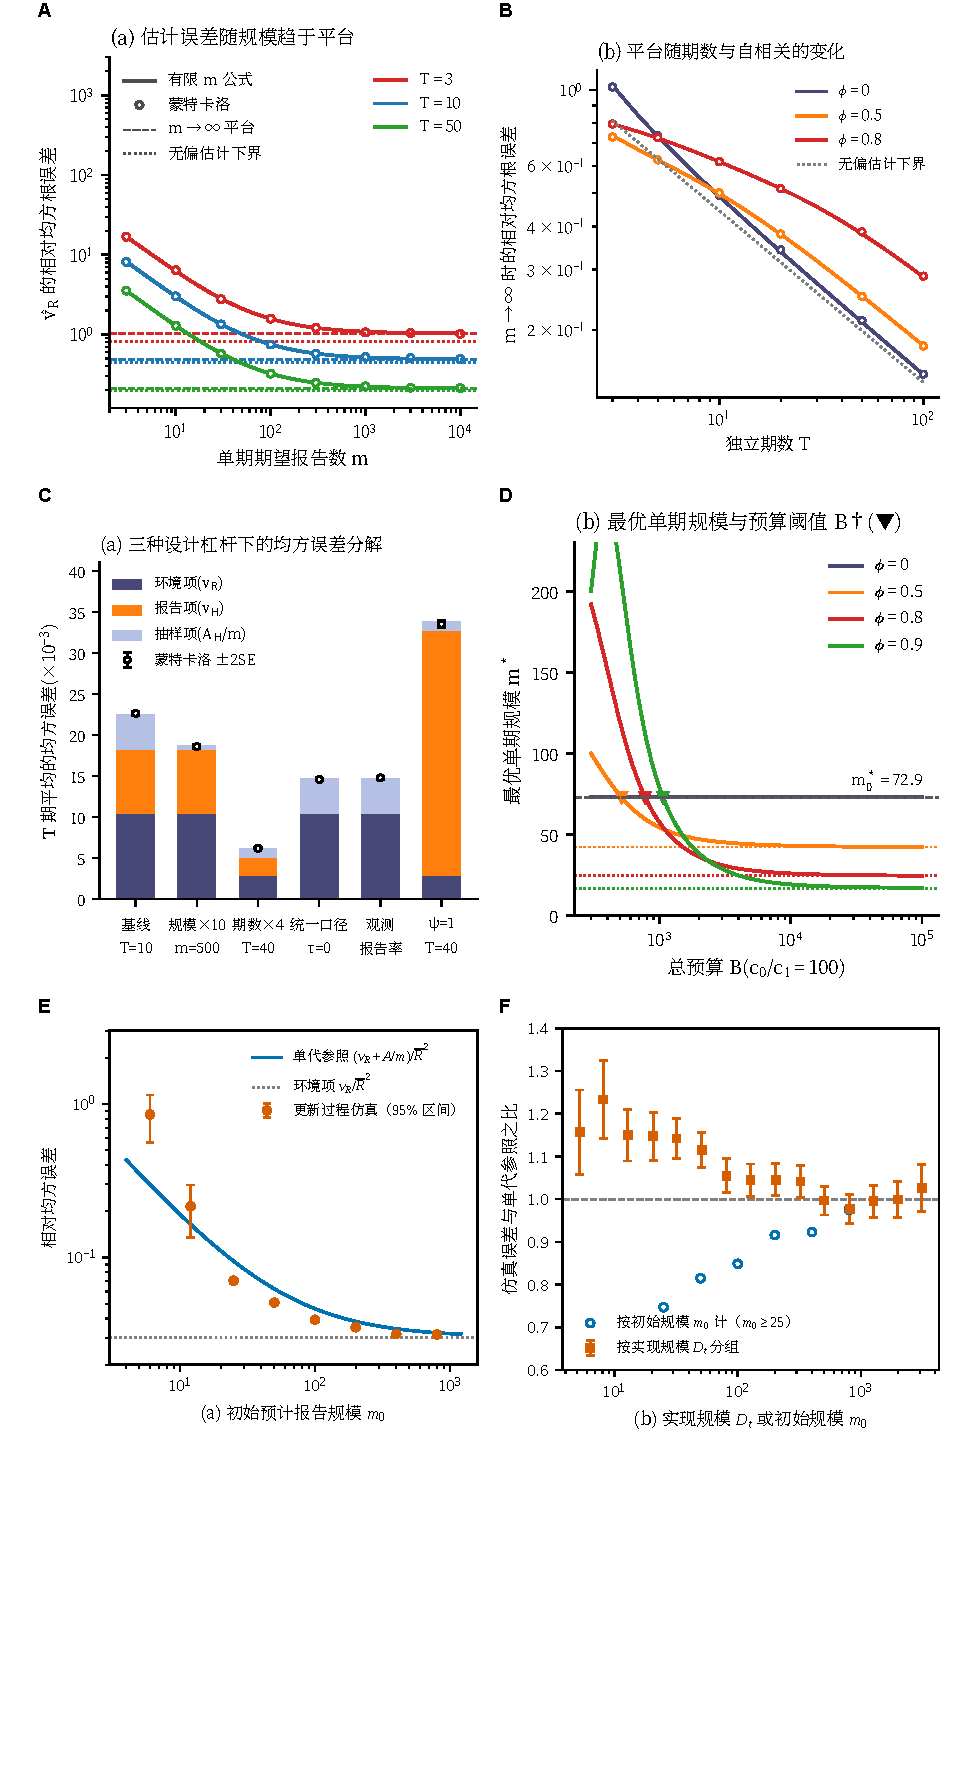
\includegraphics[width=0.865\textwidth]{figures/fig_main4.pdf}
  \caption{Estimation precision of environmental variance and surveillance design trade-offs. (A) Relative root mean squared error of the modified moment estimator $\hat{v}_R$ versus single-period sample volume $m$ across $T = 3, 10, 50$ observation periods; solid curves show analytical finite-scale formulas, circles denote 20,000 simulations, dotted lines indicate asymptotic $m \to \infty$ plateaus, and dashed lines mark Fisher information lower bounds. (B) Asymptotic variance plateau height versus period count $T$ and environmental autocorrelation $\phi$. (C) Three-way variance decomposition of $T$-period average error under varying surveillance levers (scale expansion, temporal replication, reporting standardization), with circles showing 60,000 simulations ($\pm 2$ SE). (D) Budget-constrained optimal single-period scale $m^*$ versus total budget $\mathcal{B}$ under AR(1) environments; triangles indicate the critical budget threshold $\mathcal{B}^\dagger$, dashed line marks the independent optimum $m_0^* = 72.9$, and dotted line is the asymptotic limit. (E) Relative mean squared error of growth statistics in epidemic renewal simulations versus initial scale $m_0$, compared against the single-generation reference curve $(v_R + A/m)/\bar{R}^2$ (solid curve) and environmental floor (dotted line). (F) Ratio of simulated error to theoretical reference curve across realized scale bins $D_t$.}
  \label{fig:r3-levers}
  \label{fig:design}
\end{figure}

\begin{figure}[!p]
  \centering
  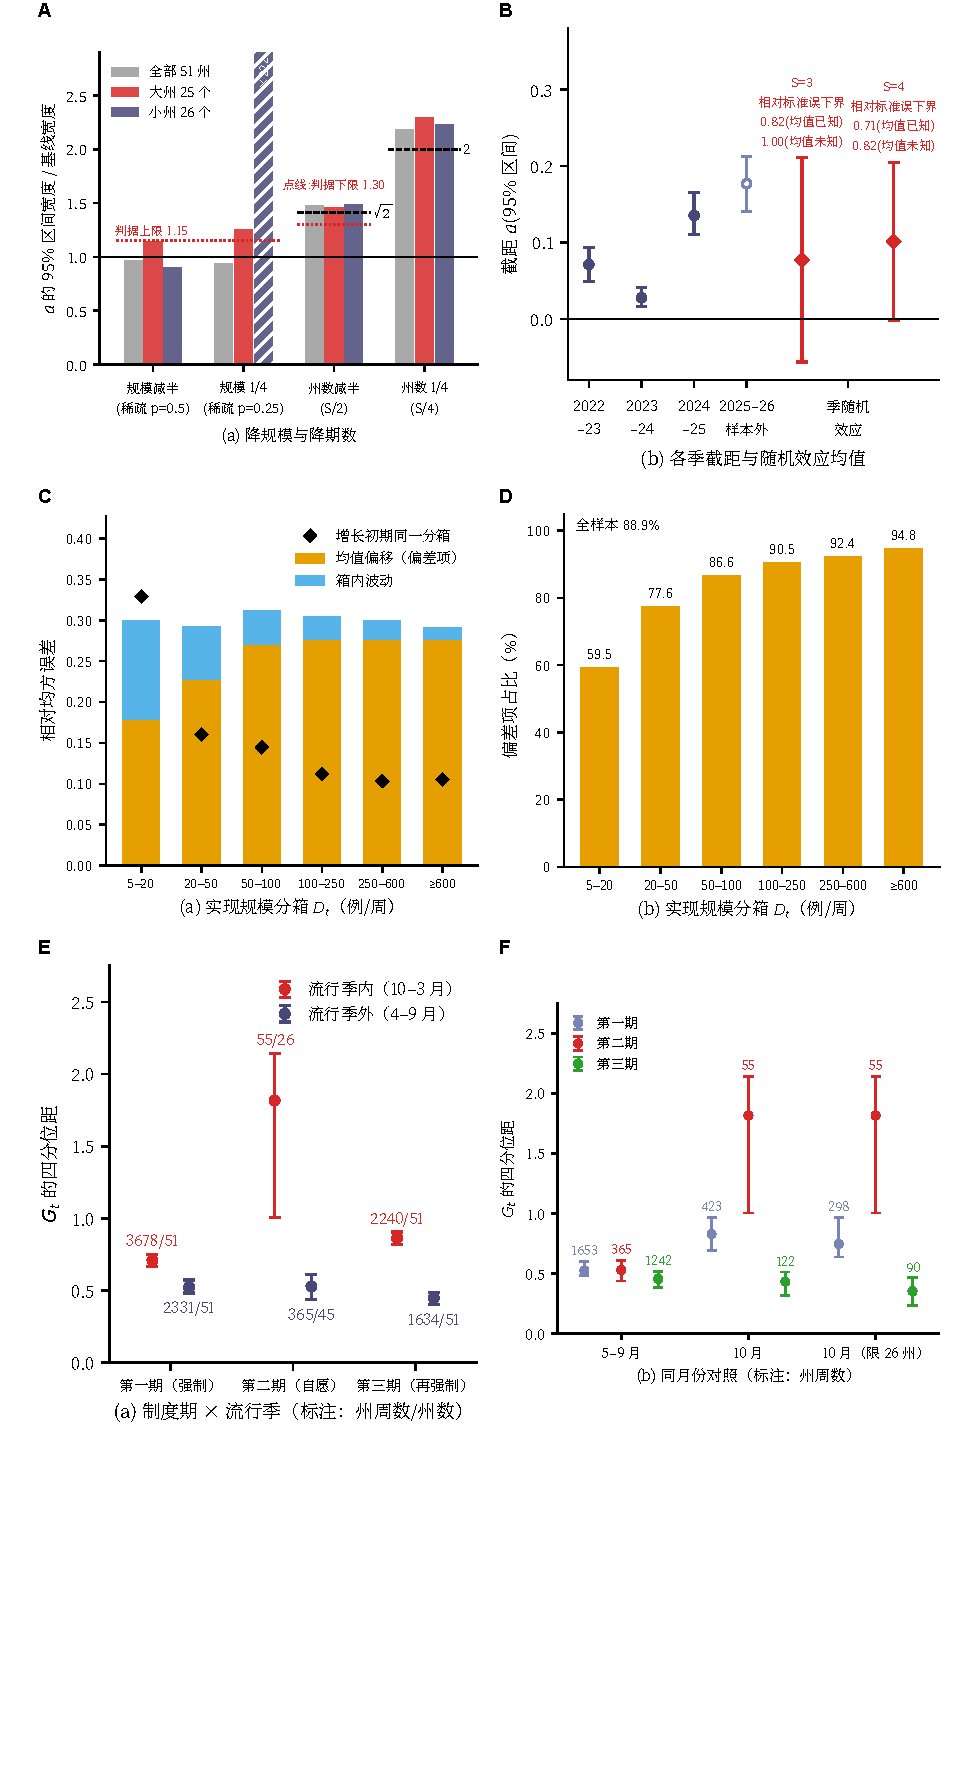
\includegraphics[width=0.91\textwidth]{figures/fig_main5.pdf}
  \caption{Season- and phase-dependent error structures in influenza surveillance. (A) Multiplier of 95\% confidence interval width for intercept $a$ under binomial thinning (sample size reduction) and state subsampling (period count reduction); dashed curve indicates the $\sqrt{S/S'}$ theoretical scaling expectation. (B) Season-specific intercepts and random-effects mean, with hollow circle denoting the out-of-sample 2025--2026 season and red labels indicating theoretical relative standard error bounds. (C) Decomposition of squared error across scale bins during peak and post-peak weeks, separating benchmark shift bias (orange) from within-bin variance (blue); diamonds denote early-phase loss. (D) Proportion of total loss explained by benchmark bias across scale bins. (E) Interquartile range of weekly growth ratios $G_t$ across three institutional reporting regimes, stratified by in-season and off-season weeks. (F) Month-matched control of growth ratio dispersion, isolating the October voluntary reporting transition.}
  \label{fig:seasons}
\end{figure}

\FloatBarrier
\section{Discussion}
\label{sec:discussion}

We have described how the error of a case-count estimate of the reproduction number depends on case volume when transmission varies between periods, offspring numbers are overdispersed and only a proportion of infections is reported. For the period-specific value, error falls without limit as reported cases accumulate. For the mean across periods and for one-step prediction, error per period approaches the environmental variance, and the balance scale $\mx=A/v_R$ marks the case volume beyond which each doubling of cases removes at most a quarter of the remaining variance. In weekly influenza hospital admissions over four seasons, an affine model gave both apparent statistics positive intercepts, although an intercept-free power law fitted the observed range about as well. Conditional on a mean generation interval of 3.6 days and on independent weekly shocks, a two-step inversion through a data-matched simulation mapped both intercepts to a latent environmental variance of about 0.04. A national-week component accounted for about 40\% to 50\% of the intercept, and facility completeness under mandatory reporting contributed less than equivalence margins of 17\% for $R_A$ and 12\% for $G$, set at a reference reporting volatility of 0.10.

The theory carries a standard result in population ecology over to surveillance data, and its general form is not new. Ecological models split the variance of population growth into a demographic term that falls with population size and an environmental term that does not \citep{engen1998demographic, lande2003stochastic}. The present model retains this partition and adds four elements that matter for surveillance. Transmission is a branching process with negative binomial offspring, so that superspreading enlarges the demographic term \citep{lloydsmith2005superspreading}. Binomial reporting adds a further term that falls with case volume, and reporting volatility adds one that does not (Proposition~\ref{prop:report-noise}). The quantity of interest is an estimate averaged over periods, so the balance scale also sets the optimal division of a budget between cases per period and number of periods (Proposition~\ref{prop:allocation}). That rule has the form of optimal allocation in two-stage sampling \citep{cochran1977sampling} and of the optimal cluster size in cluster-randomised trials \citep{raudenbush1997statistical}, with the balance scale in place of the ratio of within-unit to between-unit variance. The contribution of the present model is therefore the mapping of these terms onto the reproduction number, together with the reporting term and the calibration that links apparent weekly statistics to the latent variance, and not the variance partition itself.

The results complement the information-theoretic analyses of Parag and colleagues \citep{parag2021improved, parag2022quantifying}. Their metric for a noisy epidemic curve already contains time-varying reporting fractions, which enter through the geometric mean of the reporting probabilities, and a negative binomial extension is treated in their supplementary material \citep{parag2022quantifying}. Their target is the sequence of period-specific values, and in a Poisson renewal model the error variance of each estimate is $\Rbar/m$, so that reporting acts by rescaling the effective case count. Here the target is the mean across periods, and variation shared by all chains of transmission in a period contributes variance that is independent of $m$. The two descriptions agree at small counts and separate near the balance scale. Under the affine fit on the apparent scale of $R_A$, the fitted variance was twice the Poisson variance at 22 admissions per week and ten times at 261, and on the latent scale the corresponding values were 28 and 262. Both descriptions are therefore needed. The Poisson analysis ranks data streams by the information they carry about current transmission, and the variance partition here indicates when further cases cease to improve estimates of typical transmission.

The two-step inversion connects the apparent statistics with the latent model. The simulation first established that neither statistic estimates $v_R/\Rbar^2$ directly; the intercept of $G$ was 2.7 times this quantity and that of $R_A$ about half of it, for reasons that follow from how each statistic aggregates growth over a week. After calibration, the two statistics implied latent variances of 0.043 and 0.040 (ratio 0.93; 95\% CI 0.78 to 1.18). This consistency is expected if both statistics respond to the same latent variation and the simulation captures how each transforms it. As a test of the calibration it has limited power, since across the simulated settings it failed only when a synchronous shock to reported counts replaced the shock to transmission, in which setting the observed lag-1 autocorrelation of $G$ lay above 99\% of simulated panels. The simulated panels also reproduced the intraclass correlation and the state-level lag-1 autocorrelation of the data; the national-week share was set from the data and is not a test. Within the stated uncertainties, the calibration is therefore consistent with the empirical intercepts, under three conditions.

The first condition is the generation interval. The 3.6 days assumed by the statistics is the mean household serial interval of \citet{cowling2009estimation}, used as a proxy for the generation interval. The interval of 2.9 to 4.3 days is the 95\% confidence interval of that mean, not the range of plausible true intervals. Direct estimates of the mean generation interval, 2.8 to 3.2 days \citep{chan2025estimating}, and mean serial intervals of 2.2 and 2.8 days for influenza A subtypes \citep{vink2014serial} lie in the lower part of this interval or below it. Across true mean intervals of 2.2 to 4.3 days the implied variance ranged from 0.013 to 0.063, and at 2.9 days it was 0.026. The inversion therefore identifies $v_R$ conditionally on the interval, and its primary interval does not include uncertainty about it. If the true interval is shorter than 3.6 days, the latent variance is smaller and the latent balance scale larger, about 47 admissions per generation at 2.9 days. The second condition is independence of weekly shocks. The pooled state-level autocorrelation lay near the centre of the simulated distribution under independence and below 97\% of simulated panels with a first-order coefficient of 0.25 for $R_A$. A coefficient of 0.5 would have lowered the implied variance to about 0.026. This check concerns autocorrelation within states; the series of national-week means was not tested, and the simulated autocorrelation acted on the national and state shocks together. The third condition concerns the cross-sectional slope. The calibrated theoretical $b/a$ lies below both empirical point estimates, which fall at the 91st and 93rd percentiles of the simulated sampling distribution. With a variance-to-mean ratio of 1.5 for weekly admissions, the simulated $b/a$ rose to 68.0 for $R_A$ and 40.2 for $G$, above both empirical values, while the implied variance stayed at 0.039 and 0.044. A true generation interval of 2.9 days also reproduced the empirical $b/a$, with an implied variance of 0.026. The excess can therefore come from overdispersion smaller than a variance-to-mean ratio of 1.5, from a shorter generation interval, or from spatial aggregation (below), and these explanations imply different latent variances. The state-level autocorrelation does not favour the shorter interval, but it cannot exclude it, and the data cannot exclude a mixture of transmission and reporting shocks (Proposition~\ref{prop:report-noise}).

The fit across states also confounds case volume with spatial scale. States with more admissions are, in general, larger and more populous, and their weekly counts aggregate more local epidemics. If local environmental variation is not fully synchronised within a state, Eq.~(\ref{eq:pooling}) implies that the environmental variance of a state-level statistic falls with the number of local epidemics it contains. The relative loss would then decline with state size even if the shared term within each local epidemic were constant, and part of the slope $b$ would reflect aggregation and not sampling. Under this explanation, $b/a$ overstates the balance scale within a single reporting unit, and the design rule below applies to state-level aggregates of the size observed here. Eq.~(\ref{eq:affine}) assumes a common intercept for all states, and the data do not separate the two explanations.

Under the affine model, the empirical results are best read as a diminishing-returns scale for case volume within a period. With an apparent balance ratio of 37.4 admissions per week on the scale of $R_A$, a state that already reports at this ratio obtains half of the precision that unlimited case volume could provide, and 90\% requires nine times as many admissions. Slightly more than half of the state-weeks in the analysis windows were above the apparent ratio; the latent scale implied by the calibration is higher, so fewer state-weeks lie above it. The limit applies to case volume per period. The error of an estimate pooled over $T$ independent periods falls as $v_R/T$, estimators that shrink towards a prior mean can go below the per-period value (Appendix~\ref{app:shrinkage}), and a power law without an intercept described the observed range of scales about as well as the affine form. The balance scale is therefore a statement about where returns diminish, and it does not imply that error stops falling with more data of every kind. This interpretation is also robust to the source of the intercept. Whatever mixture of transmission, testing and statistic construction it contains, a component that is shared within a period and does not fall with case volume limits the value of further cases per period and raises the value of further periods.

The multiscale decomposition locates this component. About 41\% of the intercept of $R_A$ and 51\% of that of $G$ was common to all states in a calendar week, and resampling weeks moved the estimated intercept 1.5 to 1.9 times as much as resampling states. A national-week component cannot be reduced by scaling up surveillance in a single state, because it enters every state's loss in that week. Pooling states removes the state-specific part, and in these data pooled variance approached the national-week component, about a quarter of single-state variance, with 25 to 33 states. This share is consistent with national climatic and seasonal transmission influences \citep{cauchemez2008estimating, shaman2010absolute}, and with national changes in testing or admission practice. It is also consistent with a common trend within seasons, such as a slowing of growth as the season progresses, which is shared by all states without being week-to-week environmental variation; the present decomposition cannot separate the two. Two-way inference is required for the same reason; intervals that resample states only were about two to five times too narrow for the intercept \citep{owen2007pigeonhole, cameron2011robust}.

The contrast between reporting regimes points towards a benefit of high facility participation but does not establish it. Under mandatory reporting, a median of about 93\% of hospitals reported. Adjustment for reporting completeness changed the intercept of $R_A$ by 2\%, with a one-sided upper bound of 5.3\%, and the change was equivalent to zero within a margin of 17\%. Most state-weeks in the windows had nearly complete participation, so this bound concerns small departures from full participation, and at a reference volatility of 0.05 equivalence was not shown. During the voluntary period of 2024, when the median share fell to about 46\%, the interquartile range of log growth was 1.58 times that of the same months in 2023. The interval for this ratio, 0.95 to 2.23, includes one, and the comparison rests on a single off-season. Several checks address the main confounders. The placebo comparison of 2025 with 2023 gave 1.01, matching on reporting scale and on calendar month preserved a ratio above one, and COVID-19 and RSV admissions showed ratios above one in the same off-season, which is therefore not an independent replication. These descriptive patterns are compatible with higher empirical volatility during periods of low and variable facility participation, though they do not identify a causal effect of the reporting mandate. The adjustment measures facility participation only. Testing intensity, coding and care seeking within reporting hospitals are not captured. The laboratory proxy shared 23\% of the intercept of $R_A$, but it does not discriminate between transmission and ascertainment, because laboratory growth carries its own noise and attenuates the shared fraction towards zero.

These results suggest a design rule for routine surveillance of the mean reproduction number. Where weekly admissions per jurisdiction already exceed the price-adjusted threshold $m^*$, additional resources reduce error more when spent on further periods and on further jurisdictions whose variation is not synchronised (Eq.~(\ref{eq:pooling})) than on further cases per period. The value of complete reporting depends on the reporting volatility a system actually has. In the hypothetical example of Section~\ref{sec:res-theory}, with a relative volatility of $\tau=0.15$, standardising reporting reduced error more than a tenfold increase in case volume per period. The completeness bound observed under mandatory reporting allows $\tau$ up to about 0.056 by the scaling against the reference volatility, or about 0.040 on the latent scale (Section~\ref{sec:meth-reporting}). At $\tau=0.040$ a tenfold increase in cases reduced the mean squared error from $15.2\times10^{-3}$ to $11.4\times10^{-3}$, against $14.6\times10^{-3}$ for standardised reporting, and at $\tau=0.056$ from $15.7\times10^{-3}$ to $11.9\times10^{-3}$, against $14.6\times10^{-3}$. Under mandatory reporting, case volume therefore remained the more effective lever in this example. The value of complete reporting relative to case volume grows with the volatility that incomplete participation introduces, which the voluntary period suggests may be larger but did not establish. Seasons are the limiting unit for statements about variation between seasons. With four seasons, no unbiased estimator of a between-season variance can have a relative standard error below 0.82 (Corollary~\ref{cor:season}), and the intercept ratios for alternative denominator weights did not discriminate between mechanisms, because epidemic growth with reporting noise alone already produced $q_1<1<q_2$.

The scope of these conclusions is set by the data, the model form and the calibration. The empirical results rest on one surveillance system, four influenza seasons and rule-defined early-growth windows. The window rule was revised once and the renewal-type ratio became the primary statistic during the analysis; Table~\ref{tab:s9} lists each specification with its role and date, and the headline estimates lie within each other's intervals. The positive intercept and every quantity derived from it are conditional on the affine form, which the data did not prefer over a power law. The intercept is fitted to state-level aggregates and pools all seasons around one mean, so between-season differences in mean growth and spatial aggregation both enter it. The inversion is conditional on the generation interval, for which a household serial interval served as proxy, and on the simulated delay, offspring and independence structure. The statistic $R_A$ is a transformation of weekly growth, not a posterior estimate of $R_t$ \citep{cori2013new}. The propositions assume environmental variation that is independent between periods and a fixed number of primary cases; the renewal formulation of Section~\ref{sec:meth-loss} shows that uncertainty in infection pressure adds a further term that does not fall with case volume. The equivalence margins use the sample mean of each statistic, the null ranges for the intercept ratios in rule windows come from the calendar-window simulation, and the bin error bars in Fig.~\ref{fig:floor}B ignore clustering. Fits with state effects or stratified by state size would separate case volume from spatial aggregation, and an inversion that integrates over uncertainty in the generation interval would remove the main conditioning. Simulations with autocorrelation in the national shock alone and with the window rule applied to simulated data would test the independence assumption more directly. Renewal estimates with an explicit admission delay, hierarchical models with week effects and independent measures of testing, and a second surveillance system with mandatory reporting and more seasons would extend the empirical base.

\section{Conclusion}
\label{sec:conclusion}

The marginal value of surveillance case volume is governed by the interplay between the inferential target and intrinsic error floors. When monitoring current transmission potential, returns to sample volume do not saturate, and surveillance capacity should be determined by statistical detection power. When estimating cross-period transmission trends, expanding single-period case counts yields diminishing returns; once sample volume reaches the variance balance scale $m_\times$, additional resources should be redirected toward accumulating observation periods, expanding spatial pooling, standardizing reporting protocols, and regularly updating baseline benchmark models. Empirical analysis of US influenza hospitalisations confirms an error scaling pattern compatible with this theoretical decomposition, in which unmodelled error components account for approximately half of early-epidemic loss and cannot be explained by reporting completeness proxies, though current observations cannot separate a strict non-zero asymptote from slow decay. Resolving the scale of environmental variance requires accumulating observation periods across multiple epidemic seasons. Surveillance systems must therefore move beyond single-period sample volume as the sole metric of monitoring adequacy.


\FloatBarrier
\section{Materials and methods}
\label{sec:methods}

\subsection{Data and analysis windows}
\label{sec:meth-data}

Weekly laboratory-confirmed influenza hospital admissions and the percentage of hospitals reporting them were taken from the NHSN Weekly Hospital Respiratory Data table for the 50 US states and the District of Columbia \citep{cdc2026nhsn}, using the version retrieved on 2026-10-20. The table contained 21641 jurisdiction-weeks from 2020-08-08 to 2026-10-10. Reporting was mandatory until 30 April 2024, voluntary from 1 May to 31 October 2024 and mandatory again from 1 November 2024, giving 6009, 420 and 4077 jurisdiction-weeks with a reporting scale of at least five in the three regimes.

The primary windows covered early epidemic growth in four seasons from 2022--23 to 2025--26. Each window contained the contiguous weeks from 1 October, or from 9 November 2024 when mandatory reporting resumed, in which national weekly growth was at least 1.05, and ended the week before the first national turning point. The windows ran from 2022-10-01 to 2022-11-26, 2023-10-07 to 2023-12-23, 2024-11-09 to 2024-12-28 and 2025-10-04 to 2025-12-27, giving 42 calendar weeks. This rule replaced a first version that ended each window at the season maximum and gave only four weeks in the double-peaked 2024--25 season; the revision was made on 2026-10-20 before any intercept was fitted on the new windows. For continuity, the three calendar windows of an earlier version of this analysis (2022-10-08 to 2022-11-26, 2023-10-14 to 2023-12-16 and 2024-11-09 to 2025-01-18) were analysed as a secondary specification. A peak window contained the national peak week of each season and the seven weeks after it. No zero-imputed counts entered any window.

\subsection{Weekly growth statistics}
\label{sec:meth-stats}

Two statistics of weekly growth were computed for each state and week. The weighted growth ratio is given by:
\begin{equation}
  G_t=\frac{C_{t+1}}{D_t},\qquad D_t=0.65\,C_t+0.25\,C_{t-1}+0.10\,C_{t-2},
  \label{eq:dt}
\end{equation}
where $C_t$ is the number of admissions in week $t$ and $D_t$ is the reporting scale, with $\sum_sw_s{}^2=0.495$. Only weeks with $D_t\ge5$ were used for $G$. The renewal-type ratio converts single-week growth into a reproduction number through the generation interval \citep{wallinga2007how}, and is given by:
\begin{equation}
  R_{A,t}=\left(1+r_t\theta\right)^{\alpha},\qquad r_t=\frac{1}{7}\log\frac{C_{t+1}+0.5}{C_t+0.5},
  \label{eq:ra}
\end{equation}
where $r_t$ is the daily growth rate, and $\alpha$ and $\theta$ are the shape and scale of a gamma generation interval with mean 3.6 days and standard deviation 1.6 days, the household serial interval estimated by \citet{cowling2009estimation}. Generation intervals with means of 2.2 and 4.3 days were used as sensitivity analyses. Because the scale of $R_A$ is the single-week count, it was computed only for weeks with $C_t\ge5$ as well as $D_t\ge5$. $R_A$ is a transformation of observed growth and not a posterior estimate of $R_t$ \citep{cori2013new}; both statistics are therefore apparent quantities whose relationship to $v_R$ was established by simulation (Section~\ref{sec:meth-inversion}).

\subsection{Expected loss and the balance scale}
\label{sec:meth-loss}

In routine surveillance the number of primary cases is unobserved, and secondary infections arise from the infection pressure $\Lambda_{t+1}=\sum_{s\ge1}w_sI_{t+1-s}$ \citep{fraser2007estimating, cori2013new}. Applying the law of total variance to $C_{t+1}$ given the history $\mathcal{F}_t$, with $m=\rho\E(\Lambda_{t+1}\mid\mathcal{F}_t)$, the relative prediction variance can be written as:
\begin{equation}
  \frac{\Var(C_{t+1}\mid\mathcal{F}_t)}{m^2}=v_R+\frac{A}{m}+\mathrm{CV}^2(\Lambda_{t+1}\mid\mathcal{F}_t)\,(\Rbar^2+v_R),
  \label{eq:info-decomp}
\end{equation}
where $\mathrm{CV}$ is the coefficient of variation. The last term is a further scale-invariant component that vanishes only when infection pressure is known. For a statistic $X_t$ with mean $\bar{X}$, the relative loss $L_t=[(X_t-\bar{X})/\bar{X}]^2$ was modelled as:
\begin{equation}
  \E(L_t\mid D_t)=a+\frac{b}{D_t},
  \label{eq:affine}
\end{equation}
where, if a week were a single generation and $D_t$ were free of noise, $a=v_R/\Rbar^2$, $b=A/\Rbar^2$ and $b/a=\mx$. Binomial noise in the denominator, with relative variance $(1-\rho)\sum_sw_s{}^2/m$, increases the slope to approximately:
\begin{equation}
  b\approx\frac{A+(1-\rho)(\Rbar^2+v_R)\sum_sw_s{}^2}{\Rbar^2}.
  \label{eq:b-delta}
\end{equation}
Theoretical ranges of $b/a$ for $G$ used $\Rbar$ equal to the mean of $G$ in each specification, $v_R\in\{0.04,0.08\}$, $k\in\{0.2,0.5\}$ \citep{lloydsmith2005superspreading} and an admission probability per infection $\rho\in\{0.0056,0.021\}$ \citep{tokars2018seasonal}, with and without Eq.~(\ref{eq:b-delta}). The uncorrected balance scale over these scenarios was 21.3 to 49.2 cases.

\subsection{Estimation and inference}
\label{sec:meth-inference}

Eq.~(\ref{eq:affine}) was fitted by feasible generalised least squares with weights $1/\hat{\mu}^2$, where $\hat{\mu}$ is the fitted mean from the previous iteration, iterated to convergence \citep{wooldridge2010econometric}. Observations from the same state are dependent over time, and observations from the same week share national influences. Uncertainty was therefore estimated by a two-way bootstrap that draws states and weeks independently with replacement and weights each observation by the product of the two draw counts \citep{cameron2008bootstrap, cameron2011robust}. Each specification used 2000 bootstrap replicates with its own seed (20261024 for $R_A$ and 20261124 for $G$ in the rule windows, 20261224 for $G$ and 20261324 for $R_A$ in the calendar windows), and uncertainty is reported as the point estimate followed by the 95\% percentile interval, for example 0.0150 (95\% CI: 0.0100, 0.0208).

The intercept was decomposed by refitting Eq.~(\ref{eq:affine}) twice. The first refit removed national-week effects by using deviations from the mean across states in each week, with a small-sample factor $n_w/(n_w-1)$. The second removed additive week and state-season effects estimated by alternating projections. The national-week component is the difference between the unadjusted and week-adjusted intercepts, and the state-season component is the further change on adding state-season effects. The affine model was compared with a power law $\E(L_t\mid D_t)=cD_t{}^{-\gamma}$ by a weighted contrast of residual sums of squares, calibrated by a residual bootstrap under the power law, and by leave-one-state-out and leave-one-season-out cross-validation. Power to detect a positive intercept was computed by simulating from the fitted affine model with intercepts up to the estimated value. Sensitivity analyses of $b/a$ trimmed the most influential 1\% of losses, omitted one season at a time, used Huber weights and removed national-week effects. Further analyses used the peak window, changed the generation interval and changed the denominator weights to a single week or three equal weeks.

\subsection{Reporting completeness}
\label{sec:meth-reporting}

Coverage-adjusted statistics were computed after dividing each count by the share of hospitals reporting in that state and week. The change in intercept, $\Delta a=a-a_{\mathrm{adj}}$, was tested for equivalence to zero by two one-sided tests at the 5\% level, using 90\% intervals from a paired two-way bootstrap \citep{schuirmann1987comparison}. The margins were set at the intercept that a relative reporting volatility $\tau_0$ would add under Proposition~\ref{prop:report-noise}, and are given by:
\begin{equation}
  \delta_G=\tau_0{}^2\left(1+\frac{v_R}{\Rbar^2}\right),\qquad
  \delta_{R_A}=\kappa_A{}^2\,\tau_0{}^2\left(1+\frac{v_R}{\Rbar^2}\right),
  \label{eq:tost}
\end{equation}
where $\kappa_A=\mathrm{d}\log R_A/\mathrm{d}\log g$ propagates a perturbation of weekly growth $g$ to $R_A$, $\Rbar$ is the sample mean of each statistic, $v_R=0.04$, and $\tau_0=0.10$ (primary) or 0.05. Because $\Rbar$ is estimated, the margins expressed as shares of the intercept carry bootstrap intervals. Power was computed from a normal approximation. The interquartile range of $\log G$ and the standard deviation of $G$ over May to October were compared between 2023, 2024 and 2025. As a second proxy, $R_A$ was computed from weekly positive influenza tests in clinical laboratories for 44 states with available data, and the share of the hospital intercept removed by regressing hospital $R_A$ on laboratory $R_A$ was estimated with 500 two-way bootstrap replicates.

\subsection{Seasons and pathogens}
\label{sec:meth-seasons}

Season-specific intercepts were pooled with a DerSimonian--Laird random-effects model \citep{dersimonian1986meta}, with a $t$ interval on $S-1$ degrees of freedom for the pooled intercept and a Q-profile interval for the between-season variance \citep{viechtbauer2007confidence}. Corollary~\ref{cor:season} gives the lower bound on the precision of any between-season variance \citep{searle1992variance}. Intercept ratios $q_1=a_{(1,0,0)}/a_{w}$ and $q_2=a_{(1/3,1/3,1/3)}/a_{w}$ compare a single-week and an equal three-week denominator with the weights of Eq.~(\ref{eq:dt}). They were computed for influenza in four windows and for COVID-19 and RSV admissions in two windows each. Null ranges came from simulated epidemic growth with reporting noise but no environmental variation, over three generation intervals, three admission delays and four noise levels. Each of the eight combinations was tested on five one-sided criteria ($q_1<1$, $q_2>1$, each ratio outside its null range and a positive excess over $v_R/\Rbar^2$), and the 40 tests were adjusted by the Holm and Benjamini--Hochberg procedures \citep{holm1979simple, benjamini1995controlling}.

\subsection{Simulation of apparent statistics}
\label{sec:meth-sim}

The closed forms of Section~\ref{sec:background} were checked by Monte Carlo with 20000 replications per point. In a first, generic design, apparent weekly statistics were simulated from a daily renewal model with $\Rbar=1.2$ and the generation interval above. Weekly $R_t$ was drawn from a gamma distribution with variance $v_R$, independently across weeks, offspring were negative binomial and admissions were binomial with probability $\rho_h$ after a gamma delay with mean 5.5 days and standard deviation 3.0 days, which was assumed. Each replicate contained 500 states with initial reporting scales log-uniform between 2 and 150, four warm-up weeks and six observation weeks. Seventeen scenarios crossed $v_R\in\{0.01,0.02,0.04,0.08,0.16\}$ with $k\in\{0.1,0.35,1\}$ at $\rho_h=0.01$ and added $\rho_h\in\{0.005,0.02\}$ at the baseline, each with 20 replicates. The noise-free limit of each intercept came from a mean-field run of 20000 states in which all count noise was replaced by expectations.

\subsection{Two-step inversion}
\label{sec:meth-inversion}

The empirical intercepts were mapped to $v_R$ in two steps. In the first step, a data-matched version of the simulator gave the expected fitted intercept of each statistic as a function of $v_R$. Each simulated panel had the cross-section and length of the analysis panel, with 51 states and the four rule windows of 9, 12, 8 and 13 observation weeks. The season mean $R_s$ was the renewal-type transform of the geometric-mean national weekly growth over each window, and initial admissions in each state equalled its observed admissions in the first window week. Weekly reproduction numbers were $R_{i,s,w}=R_s+\eta_{s,w}+\varepsilon_{i,s,w}$, where the national week shock $\eta$ has variance $0.45\,v_R$ and is shared by all states, the state shock $\varepsilon$ has variance $0.55\,v_R$, and values were truncated below at 0.05. The share of 0.45 was set between the national-week shares of 0.41 and 0.51 observed for the two statistics (Section~\ref{sec:res-multiscale}); matching the simulated intraclass correlation and national-week share to the data is therefore a consistency check, and setting the share to zero or 0.65 changed the implied variance for $R_A$ from 0.040 to 0.039 and 0.040 (Table~\ref{tab:s8}). Transmission was a daily renewal process with negative binomial offspring ($k=0.35$), admissions were binomial with probability $\rho_h=0.01$ after the delay above, and both statistics were computed and filtered exactly as in the data, with the analyst's generation interval of mean 3.6 days. The design crossed $v_R\in\{0.02,0.04,0.06,0.09\}$ with 200 panel replicates per value, and Eq.~(\ref{eq:affine}) was fitted to each replicate. A calibration line $\E(\hat{a})=\gamma_0+\gamma_1v_R$ was fitted by weighted least squares with weights equal to the inverse Monte Carlo variance of each mean, and the scale factor $\kappa=\E(\hat{a})/(v_R/\Rbar^2)$ was computed with $\Rbar$ the row-weighted true mean.

In the second step, the implied variance $v_R^{\mathrm{impl}}=(a-\gamma_0)/\gamma_1$ was computed for each statistic. Its interval combined 2000 joint two-way bootstrap draws of the two empirical intercepts, which share state and week multiplicities, with independent draws of $(\gamma_0,\gamma_1)$ from their Monte Carlo sampling distribution. Agreement between the two statistics was defined as non-rejection, that is, a 95\% interval of their difference that contains zero. For the primary design, equivalence was also tested by two one-sided tests on the ratio of the implied variances with bounds of 0.80 and 1.25, using the 90\% interval of the ratio draws. Sensitivity settings changed one element of the design at a time (Table~\ref{tab:s8}). They removed the national shock or raised its share to 0.65, added first-order autocorrelation of 0.5 across weeks, set the true generation interval to a mean of 2.2 or 4.3 days while the analyst kept 3.6 days, and set the delay mean to 3.5 or 8 days. One further setting lowered $k$ to 0.1, another replaced the transmission shock by a synchronous multiplicative shock to reported counts, and the generic design above served as a bridge. Four settings added at the final revision set the true generation interval to 2.9 days, the lower end of the interval of \citet{cowling2009estimation}, set the first-order autocorrelation to 0.25, and drew weekly admissions from a gamma--Poisson mixture with a variance-to-mean ratio of 1.5 or 2.0 (Table~\ref{tab:s10}). The independence of weekly shocks was checked with the pooled lag-1 autocorrelation of $x/\bar{x}-1$ within state-season blocks of each statistic, with an interval from a state-cluster bootstrap of 1000 draws, and compared with its distribution over simulated panels at $v_R=0.04$. The calibrated theoretical $b/a$ used the same design over $v_R\in\{0.04,0.08\}$, $k\in\{0.2,0.5\}$ and $\rho_h\in\{0.0056,0.021\}$, and the range of $b/a$ across single replicates gave the distribution expected from one panel of this size. Simulation seeds were derived from 20261020 by a seed sequence indexed by setting, value of $v_R$ and replicate block; the joint bootstrap and the calibration draws used 20261921 and 20261922.



\FloatBarrier
\section*{CRediT authorship contribution statement}
\textbf{Chi Wang}: Conceptualization, Methodology, Software, Formal analysis, Data curation, Visualization, Writing - original draft, Writing - review \& editing.

\section*{Declaration of competing interest}
The author declares that they have no known competing financial interests or personal relationships that could have appeared to influence the work reported in this paper.

\section*{Funding}
This research did not receive any specific grant from funding agencies in the public, commercial, or not-for-profit sectors.

\section*{Data and code availability}
All surveillance data used in this study are publicly available from the US Centers for Disease Control and Prevention National Healthcare Safety Network (NHSN), FluSight, ILINet, FluSurv-NET, and HHS Protect. Complete analytical scripts, simulation code, and processed panel datasets required to replicate all figures and numerical findings are archived in the study GitHub repository (\url{https://github.com/wangchi2068/case-count-bottleneck}).


\FloatBarrier
\bibliographystyle{elsarticle-harv}
\bibliography{bibliography}

\end{document}
